\documentclass[10pt]{beamer}
\usetheme{Boadilla} % My favorite!
\setbeamercovered{invisible}
% To remove the navigation symbols from 
% the bottom of slides%
\setbeamertemplate{navigation symbols}{} 
\setbeamertemplate{itemize items}[default]
\setbeamertemplate{enumerate items}[default]
\xdefinecolor{lavendar}{rgb}{0.2, 0.2, 0.72}
%
\usepackage{graphicx,epsfig}
\usepackage{tikz}

%\usepackage{bm}         % For typesetting bold math (not \mathbold)
%\logo{\includegraphics[height=0.6cm]{yourlogo.eps}}
%

\newcommand{\be}{\begin{equation*}}
\newcommand{\ee}{\end{equation*}}
\newcommand{\ba}{\begin{eqnarray}}
\newcommand{\ea}{\end{eqnarray}}

\newcommand{\vso}{\vskip15pt}
\newcommand{\vst}{\vskip30pt}



\usepackage{tikz}
\usetikzlibrary{shapes,arrows,positioning}

\tikzstyle{decision} = [diamond, draw, fill=blue!20, text width=4.5em, text badly centered, inner sep=0pt]
\tikzstyle{block} = [rectangle, draw, fill=blue!20, text width=5em, text centered, rounded corners,
 minimum width=3.5cm]
\tikzstyle{line} = [draw, -latex]


\def\smallfrac#1#2{\hbox{${{#1}\over {#2}}$}}


\AtBeginSection[]
{
  \begin{frame}<beamer>{}
  \frametitle{Outline}
    \tableofcontents[currentsection]
  \end{frame}

}
\title[]{Parton Distributions for the LHC Run II}
\author{Nathan Hartland}
\institute
{
University of Oxford\\
\medskip
}

% \today will show current date. 
% Alternatively, you can specify a date.
%
\titlegraphic{\includegraphics[height=2cm]{figures/OxfordCrest.pdf}}

\date{\today}


\begin{document}
\renewcommand{\inserttotalframenumber}{34}

%%%%%%%%%%%%%%%%%%%%%%%%%%%%%%%%%%%%%%%%%%%%%%%%%%%%%%%%%
%%%%%%%%%%%%%%%%%%%%%%%%%%%%%%%%%%%%%%%%%%%%%%%%%%%%%%%%%
%%%%%%%%%%%%%%%%%%%%%%%%%%%%%%%%%%%%%%%%%%%%%%%%%%%%%%%%%
\begin{frame}
\begin{centering}
\vskip20pt
\center{\huge\color{lavendar} \textbf{Parton distributions and the LHC}}
\vskip20pt
Nathan Hartland\\

\small{University of Oxford}\\
\vso
\includegraphics[height=2.5cm]{figures/OxfordCrest.pdf}

\vskip10pt
{\bf The NNPDF Collaboration:}\\
R.~D.~Ball, V.~Bertone, S.~Carrazza, C.~Deans,\\
 L.~Del~Debbio, S.~Forte, A.~Guffanti,\\
N.H, J.I.~Latorre, J.~Rojo and M.~Ubiali. 
\vskip20pt
University of G\"ottingen\\
Friday 8th May 2015

\end{centering}

\end{frame}

%%%%%%%%%%%%%%%%%%%%%%%%%%%%%%%%%%%%%%%%%%%%%%%%%%%%%%%%%
\begin{frame}
\frametitle{What is a parton distribution function?}
\small \underline{QCD Factorisation:} \\
When considering a scattering process with a single hadron in the initial state, the calculation may be factorized into a soft part and a perturbatively calculable hard part.
\be \sigma_X(Q^2)= \sum_{a} \int_0^1 dx\; f_a(x,\mu^2)\sigma_{q_a \to X} \left( x,\frac{Q^2}{\mu^2} \right) \ee

\begin{columns}
\begin{column}{0.5\textwidth}
\includegraphics[width=\textwidth]{figures/DIS.eps}
\end{column}

	\begin{column}{0.5\textwidth}
	\begin{block}{\small $\sigma_{q_a \to X} $ - perturbative}
	\footnotesize Hard cross section for lepton scattering off a parton of flavour $a$, carrying a fraction $x$ of the parent hadron's momentum.
	\end{block}
	
	\begin{block}{\small $f_a(x,\mu^2) $ - non-perturbative}
		\footnotesize Parton distribution function describing nonperturbative dynamics of target hadron. At LO can be interpreted as the probability of finding a parton of flavour
		$a$ with momentum fraction $x$ inside the target hadron.
	\end{block}

	\end{column}
\end{columns}
\end{frame}

%%%%%%%%%%%%%%%%%%%%%%%%%%%%%%%%%%%%%%%%%%%%%%%%%%%%%%%%%

\begin{frame}
\frametitle{What is on the market?}
\small \underline{A dizzying array of options!} \\
\begin{itemize}
\item Lots of recent activity in the 'PDF industry'.
\end{itemize}

\center{Agreement between modern global sets generally very good \\ (with areas of important difference)}
\vskip10pt

\begin{columns}
\begin{column}{0.4\textwidth}
\small \textbf{Global sets:} \\
\begin{itemize}
\item NNPDF3.0 \small{  \color{lavendar} [arxiv:1410.8849]}
\item MMHT14 \small{  \color{lavendar} [arxiv:1410.3989]}
\item CT14 \small{  \color{lavendar} [preliminary]}
\end{itemize}

\small \textbf{(more) Restrictive sets:} \\
\begin{itemize}
\item ABM12 \small{  \color{lavendar} [arxiv:1310.3059]}
\item HERAPDF2.0 \small{  \color{lavendar} [preliminary]}
\end{itemize}\end{column}

	\begin{column}{0.6\textwidth}
	\includegraphics[width=\textwidth]{figures/LumiJob3.pdf}
	\end{column}
	
	
\end{columns}






\center{Comprehensive benchmarking program of newer PDF sets underway in PDF4LHC}
\end{frame}



%%%%%%%%%%%%%%%%%%%%%%%%%%%%%%%%%%%%%%%%%%%%%%%%%%%%%%%%%
\begin{frame}
\frametitle{How can we determine proton PDFs?}

\begin{columns}
\begin{column}{0.6\textwidth}
\setbeamercovered{transparent}
\begin{enumerate}
\item<1-> Theoretical input
\begin{itemize}
\item (N)NLO QCD, $\alpha_S$, HQ Treatment
\end{itemize}
\vskip15pt
\item<1-> PDF Parameterization
\begin{itemize}
\item What is a suitable choice of functional form?
\end{itemize}
\vskip15pt

\item<1-> Theoretical predictions
\begin{itemize}
\item How can we make fast pQCD predictions for experimental data while including higher order corrections?
\end{itemize}
\vskip15pt

\item<1-> Comparison to data
\begin{itemize}
\item What does (LHC) data tell us about proton structure?
\end{itemize}
\end{enumerate}
\end{column}
\begin{column}{0.3\textwidth}

\scalebox{0.6}{
      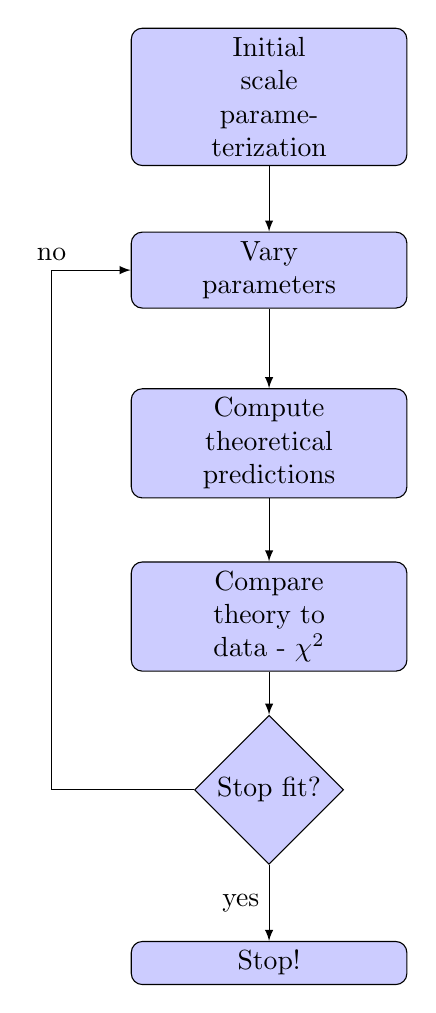
\begin{tikzpicture}[node distance=2.2cm]
        \node[block]                  (init){Initial scale parameterization};
        \node[block, below of=init]   (nbrh){Vary parameters};
        \node[block, below of=nbrh](ovgt){Compute theoretical predictions};
        \node[block, below of=ovgt]   (accp){Compare theory to data - $\chi^2$};
        \node[decision, below of=accp]   (stop){Stop fit?};
         \node[block, below of=stop]   (stopfit){Stop!};

        % invisible node helpful later
        \node[left=1cm of ovgt,scale=0.05](inv){};

        \path[line] (init) --          (nbrh);
        \path[line] (nbrh) --          (ovgt);
         \path[line] (ovgt) --          (accp);
          \path[line] (accp) --          (stop);
          
        \path[line] (stop) -- node[left]{yes}(stopfit);

       \path[-,draw] (stop) -| node{} (inv.north);
       \path[line]{} (inv.north) |- node[above]{no} (nbrh);    
           
      \end{tikzpicture}%
      }
      
      \end{column}
      
      
 \end{columns}
      \vskip10pt
\centering{In this talk $\to$ $ \chi^2[f] = \frac{1}{N_{\mathrm{dat}}}\sum_{i,j}^{N_{\mathrm{dat}}} \left( D_i - T_i[f] \right) \sigma_{ij}^{-1}  \left( D_j - T_j[f] \right)$.}



\end{frame}

%%%%%%%%%%%%%%%%%%%%%%%%%%%%%%%%%%%%%%%%%%%%%%%%%%%%%%%%%
\begin{frame}
\frametitle{What do we know from theory?}
\small \underline{Factorisation scale dependance:} \\
PDFs evolve with scale according to the DGLAP equations.
\be \mu^2 \frac{\partial f(x,\mu^2)}{\partial \mu^2} = \int_x^1 \frac{dy}{y} P\left( \frac{x}{y} \right) f (y,\mu^2)  \ee
Where $P$ are the perturbatively calculable splitting functions.

\small \underline{Theoretical constraints:} \\
\begin{itemize}
\item PDF Sum Rules
\be \int_0^1 dx\; x(\Sigma(x) + g(x)) = 1,\quad\quad   \sum_{q} \int_0^1 dx\; (q(x)-\bar{q}(x)) = 3 \ee
\end{itemize}

\begin{itemize}
\item Approx asymptotic behaviour
\be x \to 0: \quad f(x) \sim x^{\alpha}\ee
\be x \to 1: \quad f(x) \sim (1-x)^{\beta}\ee
\end{itemize}

\begin{itemize}
\item Positivity of \emph{physical observables} ($F$, $\sigma$)
\begin{itemize}
\item Beyond LO pdfs are not restricted to be positive.
\end{itemize}
\end{itemize}

\begin{center}
Aside from these constraints,\\ $x$ dependence must be determined by fitting to experimental data!
\end{center}


\end{frame}


%%%%%%%%%%%%%%%%%%%%%%%%%%%%%%%%%%%%%%%%%%%%%%%%%%%%%%%%%
\begin{frame}
\frametitle{What do we know from experiment?}
\small\underline{Many sources of precise experimental information on PDFs}
\vskip5pt

\begin{itemize}
\item The \textbf{backbone} - DIS data

\begin{itemize}
\item Large fixed-target DIS datasets available from SLAC/BCDMS/NMC.
\item Precise, clean data from HERA.
\item NC data constrains quark singlet, gluon distributions. \\CC data gives a handle on light flavour separation.
\item $\nu$-DIS data (still) provides most of the constraints upon strange distributions.
\end{itemize}
\vskip5pt

\item \textbf{Flavour separation} - Drell-Yan data

\begin{itemize}
\item Low-energy fixed-target data from FNAL
\item Tevatron and LHC data providing important constraints.
\end{itemize}
\vskip5pt
\item \textbf{Large-x gluon} - Inclusive jet data (also $t$-production)

\begin{itemize}
\item Substantial constraints from Tevatron/LHC inclusive jet measurements.
\item $t\bar{t}$ data becoming more important.
\end{itemize}

\end{itemize}
\end{frame}

%%%%%%%%%%%%%%%%%%%%%%%%%%%%%%%%%%%%%%%%%%%%%%%%%%%%%%%%%
\begin{frame}
\frametitle{Dataset selection - kinematic coverage}
\begin{center}
\includegraphics[width=0.9\textwidth]{figures/23kin.pdf}
\end{center}
\end{frame}

%%%%%%%%%%%%%%%%%%%%%%%%%%%%%%%%%%%%%%%%%%%%%%%%%%%%%%%%%
\begin{frame}
\frametitle{Parton distribution fitting - initial scale parameterization}
\begin{itemize}
\item PDFs at the initial scale are parametrised by some functional form
\end{itemize}

\begin{columns}
\begin{column}{0.5\textwidth}
\begin{block} {\centering \small Typical Parameterisations}
\begin{itemize}
\item<1-> \small MSTW08 $\sim$ 28 total PDF parameters 
\end{itemize}
    \be f_v(x) \sim ax^{b}(1-x)^{c}(1+d\sqrt{x}+e x),\ee   \begin{itemize}
\item<1-> \small CT10   $\sim$ 26 total PDF parameters 
	\end{itemize}
	\small \be f_v(x) \sim ax^b(1-x)^c \exp{(dx + ex^2 + f\sqrt{x})}.\ee \begin{itemize}
\item<1-> \small HERAPDF   $\sim$ 10 total PDF parameters 
	\end{itemize}
		\small \be f_v(x) \sim ax^b(1-x)^c \exp{(1+dx + ex^2)}.\ee

\end{block}

\begin{block}
{ \small \centering NNPDF functional form}
\begin{itemize}
\item<1-> \small NNPDF $\sim$ 259 total PDF parameters 
\end{itemize}
\be f(x) \sim ax^b(1-x)^{c} \mathrm{NN}(x). \ee
\end{block}
\end{column}
	\begin{column}{0.4\textwidth}
	\small 
	
\begin{itemize} \small
\item<1-> Attempt to minimise figure of merit by varying ($a$..$f$).
\item<1-> Choice of functional form: Parameterization \emph{bias}
\end{itemize}
\vskip10pt
\begin{center}
\underline{NNPDF Strategy}\end{center}
\vskip-10pt
\begin{itemize} \small
\item<1-> Minimise bias by choosing extremely flexible functional form
\item<1-> Each PDF parametrized by a 2-5-3-1 Neural Network
\item<1-> 259 Free parameters $\to$ \textbf{massively redundant} parameterization
\item<1-> $b,c$  $\to$ randomised preprocessing .

\end{itemize}

\end{column}
\end{columns}
\end{frame}


%%%%%%%%%%%%%%%%%%%%%%%%%%%%%%%%%%%%%%%%%%%%%%%%%%%%%%%%%
\begin{frame}
\frametitle{Theoretical Predictions}
Calculate theoretical predictions for comparison with experimental data.\\
Evolve to required scale and perform convolution with hard coefficients.\\
\vskip10pt
\underline{DIS data:} cross sections parametrized in terms of  \textbf{structure functions}:
\be F_i(x,Q^2) = \int\frac{dy}{y} C_{i}^{j}(y,\alpha_s(Q^2))f_j\left(\frac{x}{y},Q^2\right) \ee

\underline{Hadron Collider data:} perform double convolution over PDFs
\be \sigma_X= \sum_{a,b} \int_0^1 dx_1dx_2 f_a(x_1,Q^2)f_b(x_2,Q^2)\sigma_{q_aq_b \to X} \left( x_1,x_2,Q^2 \right) \ee
Hadronic data dependant upon PDFs through parton-parton luminosities:
\be \Phi_{ij}(\tau,M_X^2) = \frac{1}{s}\int_\tau^1\frac{dx_1}{x_1} f_i(x_1,M_X^2)f_j(\tau/x_1,M_X^2) \ee

\end{frame}


%%%%%%%%%%%%%%%%%%%%%%%%%%%%%%%%%%%%%%%%%%%%%%%%%%%%%%%%%
\begin{frame}
\small
\frametitle{Minimisation and Stopping in NNPDF}
\textbf{Minimisation by genetic algorithms}\\
\underline{Problem}: Very large parameter space, $\chi2$ highly nonlocal. \begin{itemize}
\item<1-> Minimisation is challenging.
\end{itemize}\underline{Solution}: Genetic Algorithms (GA)
\begin{itemize}
\item<1-> Generate mutations of fit parameters.
\item<1-> Select those mutations that minimise figure of merit.
\end{itemize}
\vskip10pt
\textbf{ Dynamical fit stopping by cross-validation}\\
\underline{Problem}:  extremely flexible parameterisations are prone to \emph{overfitting}.
\\
\begin{itemize}
\item<1->Fit has so many parameters, the minimum $\chi^2$ corresponds to a fit not only to
the data, but also statistical noise.
\end{itemize}
\underline{Solution}:  dynamical stopping by \emph{Cross Validation}.
\begin{itemize}
\item<1-> Split the dataset into a training set and a validation set.
\item<1-> Use the training set for minimisation, monitor the $\chi^2$ to the validation set.
\item<1-> Stop the fit when the $\chi^2$ to the validation set starts to increase while
the $\chi^2$ to training set is still decreasing.

\end{itemize}
\end{frame}

\begin{frame}
\frametitle{Cross-validation stopping}
	\begin{center}
   \includegraphics[width=0.9\textwidth]{figures/lookbackchi2prof.pdf}
   \end{center}
 \end{frame} 


%%%%%%%%%%%%%%%%%%%%%%%%%%%%%%%%%%%%%%%%%%%%%%%%%%%%%%%%%
\begin{frame}
\frametitle{Standard approach to parton fitting - uncertainties}
How to propagate uncertainties from the experimental data to the PDFs?
\underline{Standard Approach}: Linear propagation of uncertainties by Hessian Method.
\begin{itemize}
		\item<1->For a set of fit parameters $\{ a\} $ define a tolerance in $\chi^2$:
		\be \Delta\chi^2(a) \equiv \chi^2(a) - \chi^2(a^\mathrm{min}) = \sum^n_{i,j=1}H_{ij}(a_i-a_i^\mathrm{min})(a_j - a_j^\mathrm{min}). \ee
		\item<1-> Determine PDFs on surface of constant $\Delta\chi^2=T$ in parameter space.
		\begin{itemize}
			\item<1-> Numerical difficulties: Need to use rescaled eigenvectors of $H$.
		\end{itemize}
		\item<1-> Obtain $2n$ PDF sets $S_i^\pm$, where $n$ is the number of free parameters in the fit. \vso
		\item<1-> Uncertainty in an observable $\mathcal{O}$ given by:
		\be \mathrm{Var}[\mathcal{O}] = \frac{1}{2}\sum_{i=0}^n (\mathcal{O}[S_i^+] - \mathcal{O}[S_i^-] )^2.\ee
\end{itemize}

\end{frame}


%%%%%%%%%%%%%%%%%%%%%%%%%%%%%%%%%%%%%%%%%%%%%%%%%%%%%%%%%
\begin{frame}
\frametitle{Monte Carlo uncertainty determination}
\begin{itemize}
\item<1->Form an ensemble of $N$ artificial data 'replicas' by importance sampling the original data set.
\\
\item<1->The ensemble of artificial data replicas forms a representation of the probability distribution in data.
\\
\item<1->Perform a separate fit to each data replica, obtain an ensemble of PDF replicas.
\\
\end{itemize}
 \begin{figure}[b!]
    \begin{center}
      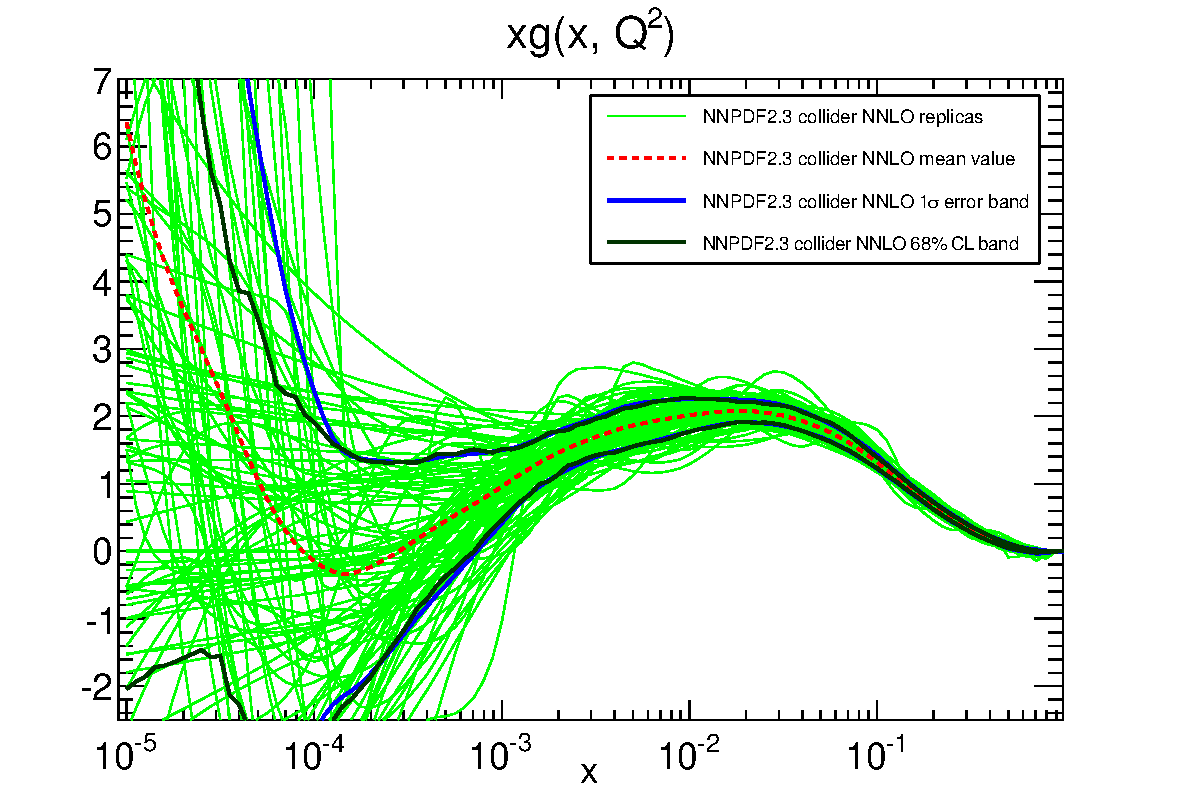
\includegraphics[width=0.45\textwidth]{figures/xg_rep_Q_2_log-23coll-nnlo.pdf}
      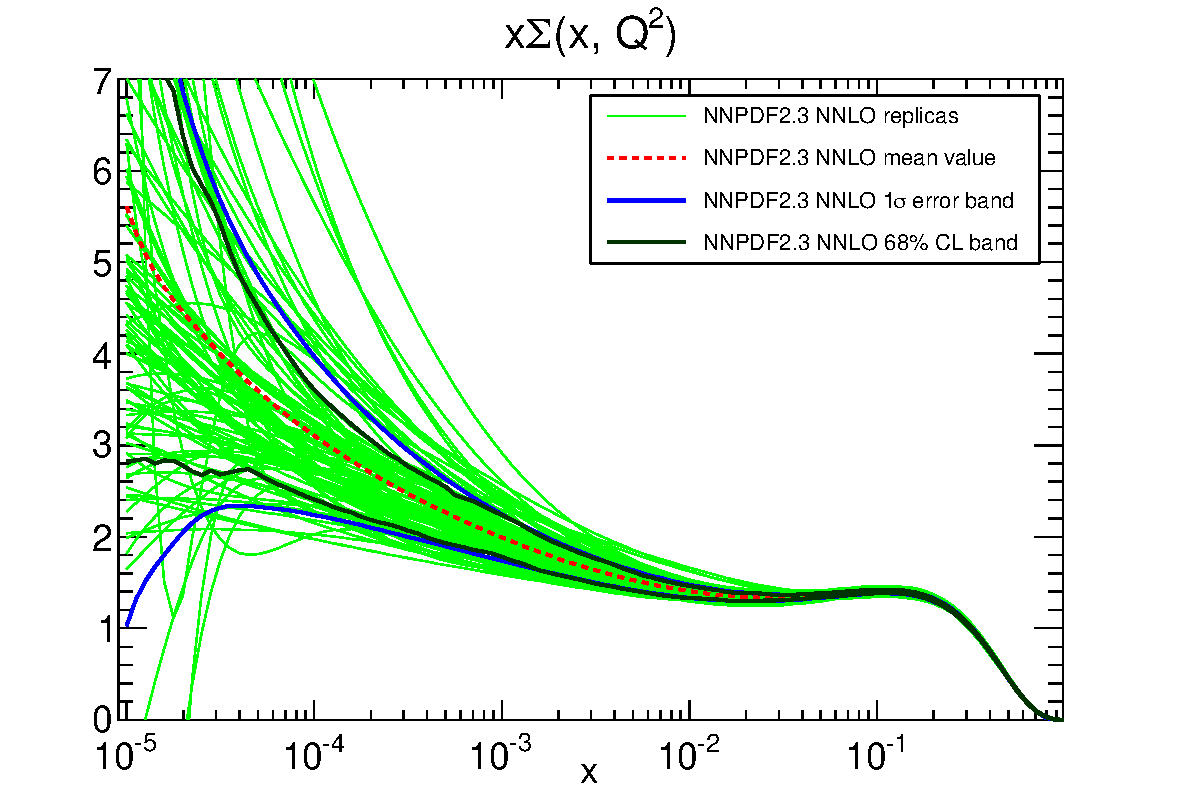
\includegraphics[width=0.45\textwidth]{figures/xSinglet_rep_Q_2_log-23-nnlo.pdf}
    \end{center}
    \vskip-0.5cm
    \label{fig:pdf-jets}
\end{figure}

\end{frame}

%%%%%%%%%%%%%%%%%%%%%%%%%%%%%%%%%%%%%%%%%%%%%%%%%%%%%%%%%
\begin{frame}
\frametitle{NNPDF User Guide}

\begin{columns}
\begin{column}{0.4\textwidth}
\small
\begin{block} 
{ \small Central value predictions}
		\small \be \langle\mathcal{O}\rangle=\smallfrac{1}{N}\,\sum_{k=1}^{N}\mathcal{O}[f_k]\, .\ee
\end{block}
\vskip5pt
\begin{block}
{\small Uncertainties }
	\small	\be {\mathrm{Var}}[\mathcal{O}]=\smallfrac{1}{N}\,\sum_{k=1}^{N}(\mathcal{O}[f_k] -  \langle\mathcal{O}\rangle )^2 .\ee
\end{block}
\end{column}

\begin{column}{0.6\textwidth}
      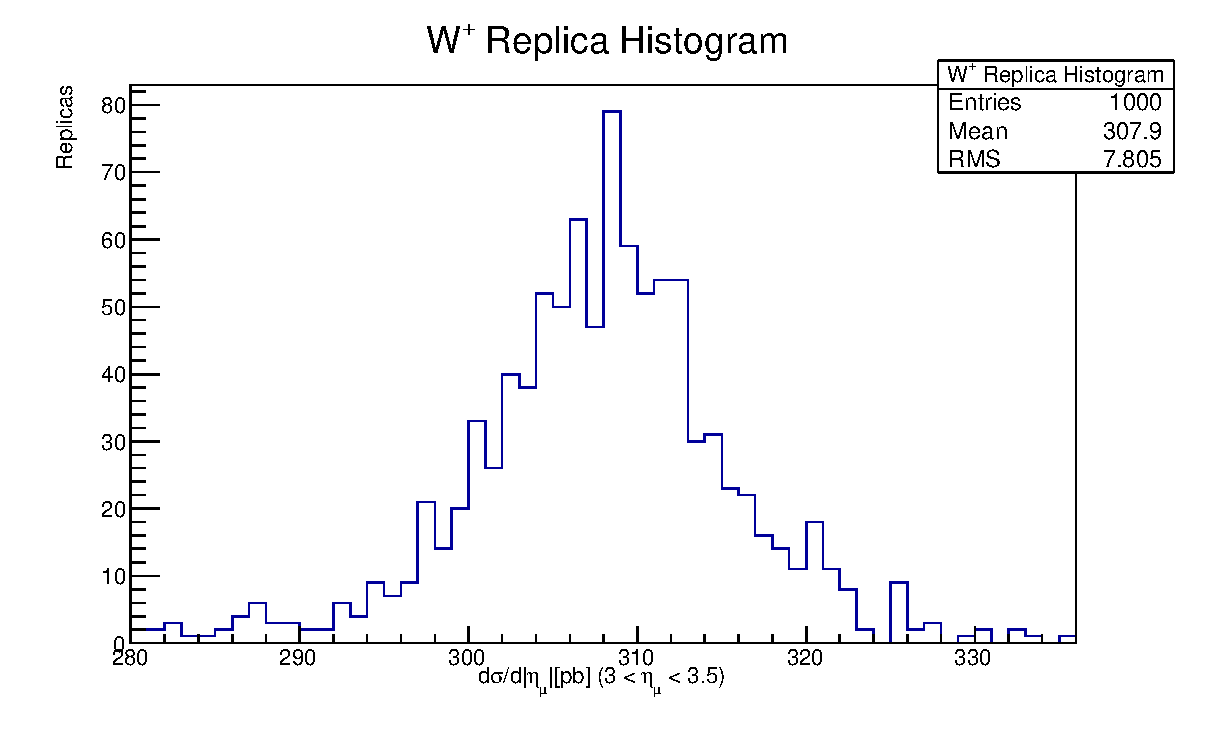
\includegraphics[width=\textwidth]{figures/WpHist.eps}
\end{column}
\end{columns}

\vso
\center{Uncertainties in the PDFs faithfully represent the experimental data. \\No tolerance criterion is required.}

\end{frame}




%%%%%%%%%%%%%%%%%%%%%%%%%%%%%%%%%%%%%%%%%%%%%%%%%%%%%%%%%
\begin{frame}
\frametitle{Parton distributions in the LHC era}
\underline{Run-I LHC data has provided a \emph{wealth} of information on parton distributions. }
\vskip5pt	
\begin{itemize}
\item \textbf{NNPDF2.2} (2011) $\to$ First (trial) inclusion of LHC data into PDF fits 
\item \textbf{NNPDF2.3} (2012) $\to$ First comprehensive analysis including all available pdf-sensitive LHC data.

\end{itemize}
\includegraphics[width=0.50\textwidth]{figures/ATLASR04JETS36PB_2.eps}
\includegraphics[width=0.50\textwidth]{figures/MSTWcompareatlas.pdf}
\vskip15pt
LHC data has also provided many \textbf{challenges} for PDF fitters
\end{frame}

%%%%%%%%%%%%%%%%%%%%%%%%%%%%%%%%%%%%%%%%%%%%%%%%%%%%%%%%%
\begin{frame}
\frametitle{What can the LHC tell us?}
\begin{columns}
\begin{column}{0.5\textwidth}
\includegraphics[width=\textwidth]{figures/Collider_comp.pdf}
\end{column}
\begin{column}{0.5\textwidth}
LHC Constraints available upon almost \\ all PDF combinations.

\vskip10pt
\textbf{\underline{Key areas}}\\
\begin{itemize}
\item Valence distributions
\item Light flavour separation
\item Strangeness
\end{itemize}
\end{column}
\end{columns}

\begin{center}
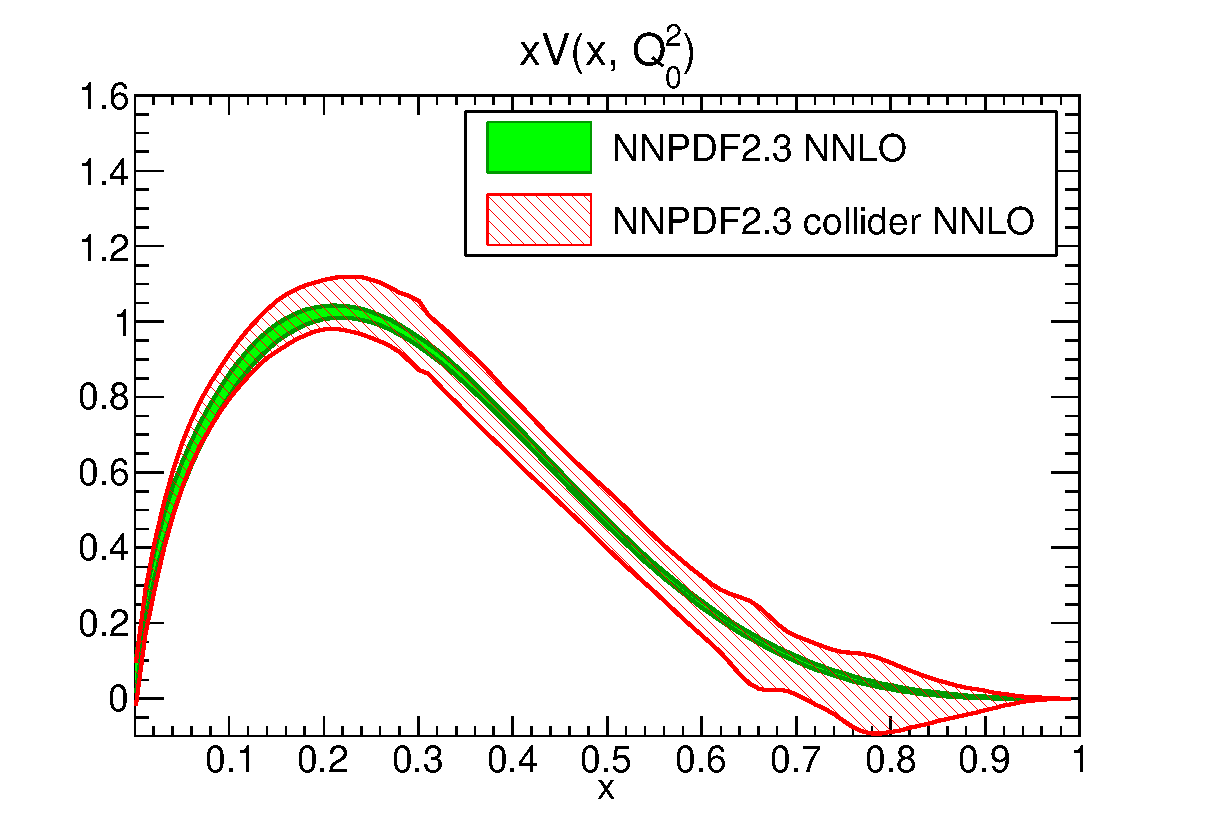
\includegraphics[width=0.50\textwidth]{figures/xV_Q_2_lin-23-vs-23coll-nnlo.eps}
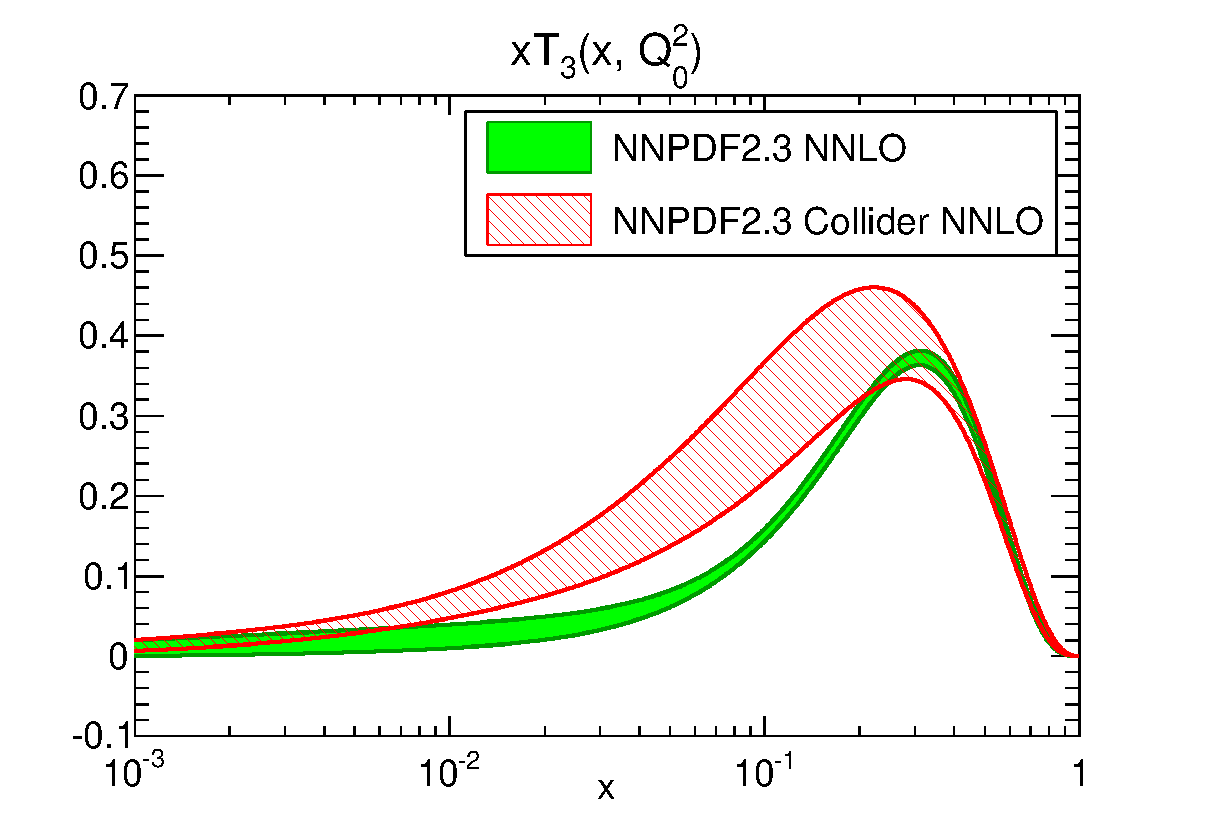
\includegraphics[width=0.50\textwidth]{figures/xT3_Q_2_log-23-vs-23coll-nnlo.eps}\\
\end{center}
\end{frame}

%%%%%%%%%%%%%%%%%%%%%%%%%%%%%%%%%%%%%%%%%%%%%%%%%%%%%%%%%
\begin{frame}
\frametitle{Parton distributions ready for Run-II}
\underline{Are our results and methodology good enough?}

\begin{itemize}
\item Can we take \emph{full advantage} of the available experimental datasets?
\item Do we have the computational tools required to include a large (and ever-expanding) LHC dataset?
\item How can we best verify that our methodology is robust?
\end{itemize}
\vskip15pt
\underline{For NNPDF3.0 every point of the methodology has been revisited.}

\begin{itemize}
\item Fitting code re-written from scratch in modern, modular C++.
\item Make use of efficient computational tools to include \textbf{all relevant and available LHC data}.
\item Thorough examination of fitting procedure through the lens of \emph{closure tests}.
\end{itemize}
\end{frame}

%%%%%%%%%%%%%%%%%%%%%%%%%%%%%%%%%%%%%%%%%%%%%%%%%%%%%%%%%
\begin{frame}
\frametitle{Computation tools for PDF fits}

How can we efficiently include LHC data into a full fit?

\underline{Tools}: APPLgrid/FastNLO projects 

\begin{itemize}
\item<1-> Precompute and store MC weights on an interpolation grid in $x$ and $Q^2$:
\end{itemize}
 \be \sigma= \sum_p \sum_{l}^{N_{\mathrm{sub}}} \int_0^1 dx_1dx_2\; \hat{\sigma}^{(p)(l)} \left( x_1,x_2,Q^2 \right)  F^{(l)}\left(x_1, x_2,  Q^2 \right) \to \ee

\begin{equation}
\label{eq:applconv}
\sigma = \sum_p \sum_{l}^{N_{\mathrm{sub}}} \sum_{\alpha,\beta}^{N_x} \sum_{\tau}^{N_{Q}}
W_{\alpha\beta\tau}^{(p)(l)} \,
F^{(l)}\left(x_{\alpha}, x_{\beta},  Q^2_{\tau}\right)
\end{equation}

\begin{itemize}
\item<1-> Interpolating interfaces to \textbf{automated} NLO codes have recently arisen.
\end{itemize}

\begin{columns}
\begin{column}{0.6\textwidth}
\includegraphics[width=0.50\textwidth]{figures/100MDYMSTWPlot.pdf}
\includegraphics[width=0.50\textwidth]{figures/tt_yt_hs.jpg}
\end{column}
\begin{column}{0.4\textwidth}
\textbf{\underline{MCgrid} [Del Debbio et al.]}\\
{\small SHERPA $\to$ APPLgrid/FastNLO}\\
\vskip10pt
\textbf{\underline{aMCfast} [Bertone et al.]}\\
{\small aMC@NLO $\to$ APPLgrid }

\end{column}
\end{columns}

\end{frame}

%%%%%%%%%%%%%%%%%%%%%%%%%%%%%%%%%%%%%%%%%%%%%%%%%%%%%%%%%
\begin{frame}
\frametitle{Computation tools for PDF fits $\to$ FastKernel}

\begin{equation}
\label{eq:applconv}
\sigma = \sum_p \sum_{l}^{N_{\mathrm{sub}}} \sum_{\alpha,\beta}^{N_x} \sum_{\tau}^{N_{Q}}
W_{\alpha\beta\tau}^{(p)(l)} \,
F^{(l)}\left(x_{\alpha}, x_{\beta},  Q^2_{\tau}\right)
\end{equation}
APPLgrid/FastNLO are fast, but \textbf{not fast enough} for NNPDF fits.\\
\underline{Idea}: Combine weight grids with evolution grids for best performance.
\be f_i(x_{\alpha},Q^2_\tau) =  \sum_\beta^{N_{x}} \sum_{j}^{N_{\mathrm{pdf}}} A^{\tau}_{\alpha\beta ij}N^0_j(x_{\beta} ) \quad \to \quad
 \sigma= \sum_{\alpha,\beta}^{N_x}\sum_{i,j}^{N_{\mathrm{pdf}}} \sigma_{\alpha\beta i j}N_i^0(x_\alpha)N_j^0(x_\beta)
\ee 
 \begin{itemize}
\item<1-> Precomputing all $Q^2$ dependence leads to extremely efficient calculations.
\end{itemize}

\begin{table}
\begin{center}
\textbf{Speed per datapoint of convolution methods}
\begin{tabular}{|c|c|c|c|c|}
\hline Observable &{\small\sc APPLgrid} & {\small\sc FK} & optimized  {\small\sc FK} \\
\hline $W^+$ production &1.03 ms & 0.41 ms (2.5x) & 0.32 ms (3.2x) \\
\hline Inclusive jet production &2.45 ms & 20.1 $\mu$s (120x) & 6.57 $\mu$s (370x) \\ 
\hline
\end{tabular}
\end{center}
\end{table}

\end{frame}

%%%%%%%%%%%%%%%%%%%%%%%%%%%%%%%%%%%%%%%%%%%%%%%%%%%%%%%%%
\begin{frame}
\frametitle{Dataset for NNPDF3.0}
With these computational tools, we could considerably expand the dataset.\\
\vskip10pt

\begin{columns}
  \begin{column}{0.5\textwidth}
  
	\underline{HERA-II}
	\begin{itemize}
	\item H1 large $Q^2$ data (NC+CC).
	\item H1 low $Q^2$, large $y$ data (NC).
	\item ZEUS positron beam data (NC+CC).
	\item HERA combined $F^2_c$ data.
	\end{itemize}
	\vskip 10pt
	\underline{LHCb}
	\begin{itemize}
	\item $Z \to ee$ large-$y$.
	\end{itemize}
	
\end{column}

  \begin{column}{0.5\textwidth}
  
          \underline{ATLAS}
  	  \begin{itemize}
	  	\item $\sqrt(s)$ = 2.76 TeV inclusive jets.
		\item High mass Drell-Yan.
	  \end{itemize}
	\vskip 10pt 
	\underline{CMS}
	\begin{itemize}
	\item Inclusive jets at $\sqrt{s}$ = 7 TeV.
	\item Double diff. Drell-Yan.
	\item $W$ $\mu$ charge asymmetry.
	\item $W+c$.
	\end{itemize}
	
\end{column}

\end{columns}
\vskip 15pt
i.e all relevant data available (with correlation information) at the time

\end{frame}

%%%%%%%%%%%%%%%%%%%%%%%%%%%%%%%%%%%%%%%%%%%%%%%%%%%%%%%%%
\begin{frame}
\frametitle{Dataset for NNPDF3.0}
\begin{center}
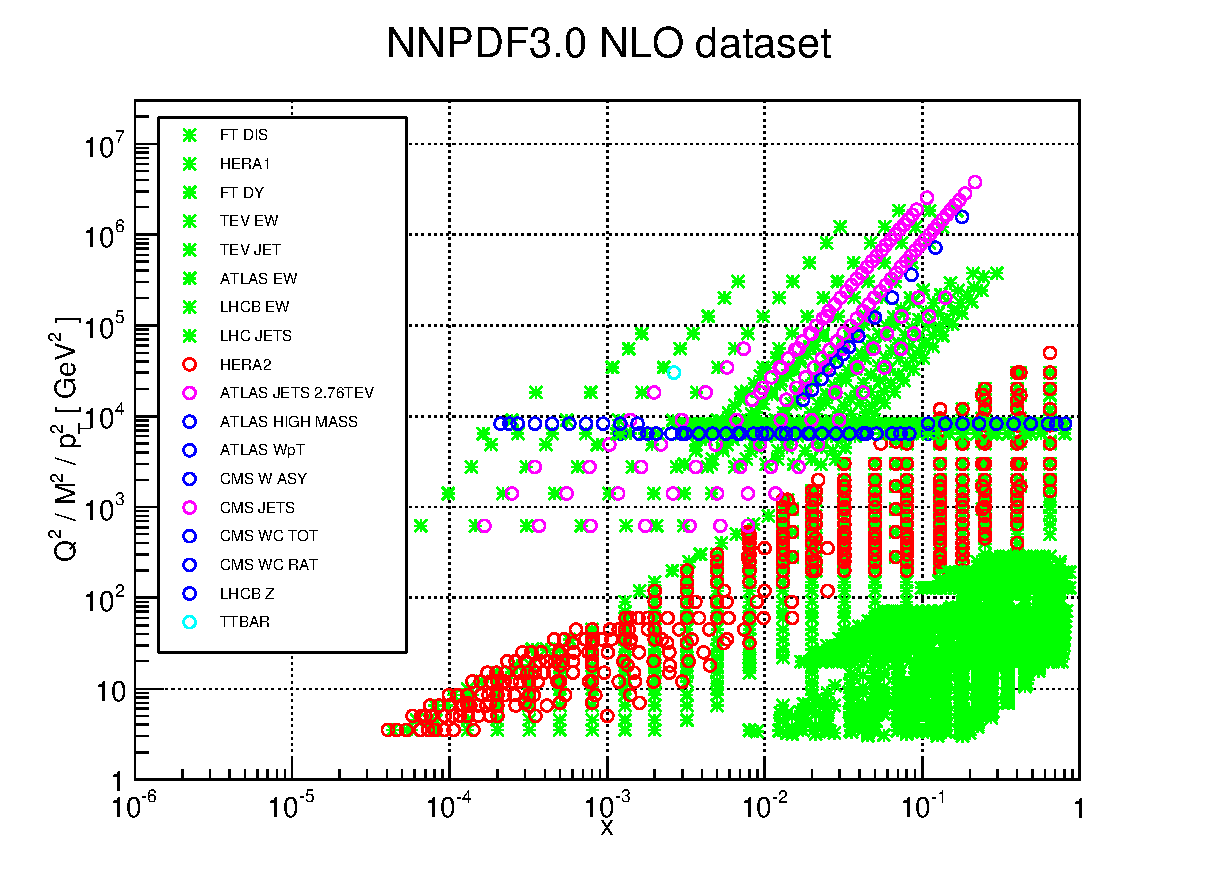
\includegraphics[width=0.8\textwidth]{figures/30kin.eps}\\
\textbf{4276} total datapoints (\textbf{471} from the LHC).
\end{center}
\end{frame}

%%%%%%%%%%%%%%%%%%%%%%%%%%%%%%%%%%%%%%%%%%%%%%%%%%%%%%%%%

\begin{frame}
\frametitle{Methodology for NNPDF3.0}
How do we ensure that our fit minimises \emph{bias}?\\
\emph{Related studies by Thorne-Watt [arXiv:1205.4024]}
\vskip15pt
\underline{Perform a \textbf{Closure Test}}:

\begin{itemize}
\item<1-> \textbf{Generate artificial pseudo-data based upon a known PDF distribution.}\\
		\small Pseudodata generated according to NLO pQCD. Dataset is therefore free of internal inconsistencies.
		\vskip15pt
		
\item<1-> \textbf{Simulate experimental noise in the pseudodata. }\\
			\small Data points perturbed according to multi-gaussian distribution defined by the experimental
			covariance matrix.
			\vskip15pt
\item<1-> \textbf{Perform a full PDF fit to the pseudo-dataset.}\\
		\small Closure fit should recover generating PDF up to the level of experimental uncertainty. Reproduction must be (reasonably) independent of generating PDF.
\end{itemize}

\end{frame}


%%%%%%%%%%%%%%%%%%%%%%%%%%%%%%%%%%%%%%%%%%%%%%%%%%%%%%%%%
\begin{frame}
\frametitle{Methodology for NNPDF3.0}
{\small Pseudodata categorised into three 'levels' corresponding to the $\chi^2$ of a perfect fit. }
\begin{itemize}
\item Level zero - perfect pseudodata with no fluctuations.
\item Level one  - pseudodata with fluctuations according to $\sigma$.
\item Level two  - pseudodata with fluctuations \textbf{and} MC replicas.
\end{itemize}

\begin{center}
\includegraphics[width=0.7\textwidth]{figures/closuretest_levels.pdf}\\
\end{center}

\end{frame}

%%%%%%%%%%%%%%%%%%%%%%%%%%%%%%%%%%%%%%%%%%%%%%%%%%%%%%%%%
\begin{frame}
\frametitle{Level zero closure tests}

\begin{columns}
  \begin{column}{0.5\textwidth}
  \begin{itemize}
  \item Level zero tests - $\chi^2 \sim 0$
  \item Determines fitting flexibility
  \item Tests \emph{extrapolation uncertainty} 
  \end{itemize}
  \vskip15pt
  \underline{\small Ideal environment for tuning minimisation.}
   \end{column}
  
    \begin{column}{0.5\textwidth}
 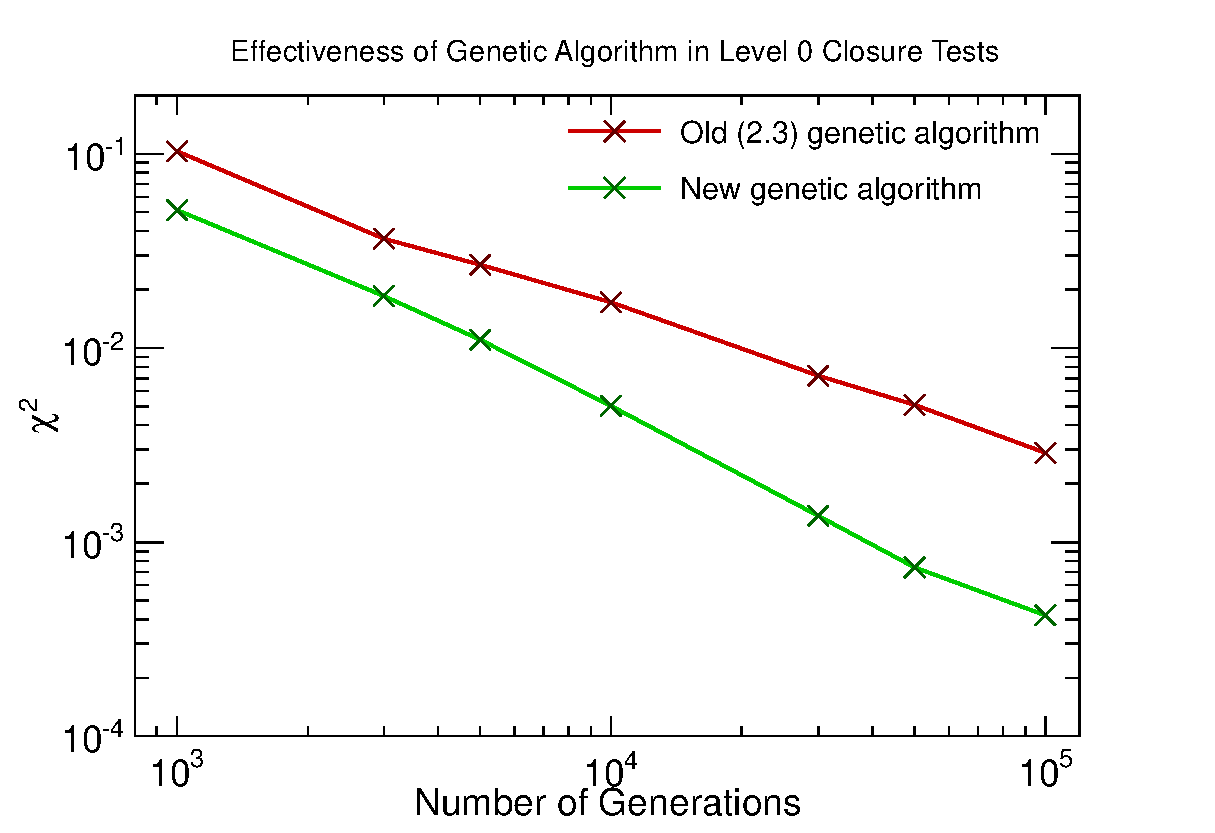
\includegraphics[width=0.8\textwidth]{figures/chi2vslength.eps}\\

  \end{column}  
  \end{columns}


\begin{center}
\includegraphics[width=0.4\textwidth]{figures/xu-ctlvl0_vs_MSTW_initscale.eps}
\includegraphics[width=0.4\textwidth]{figures/xubar-ctlvl0_vs_MSTW_initscale.eps}

\end{center}

\end{frame}

%%%%%%%%%%%%%%%%%%%%%%%%%%%%%%%%%%%%%%%%%%%%%%%%%%%%%%%%%
\begin{frame}
\frametitle{Level zero closure tests - preprocessing}

\begin{center}
\underline{Tests provided important information of the sensitivity of our fits to \emph{preprocessing}}
\end{center}


$ \mathrm{Recall:} \quad f(x) \sim x^{-\alpha}(1-x)^{\beta} P(x).$

\begin{itemize}
\item NNPDF2.3 $\to$ preprocessing randomised within a fixed range of values.
\item NNPDF3.0 $\to$ range is iteratively improved on a fit-by-fit basis.

\end{itemize}

\begin{center}
$\alpha_{\mathrm{eff}}(x) = \ln f(x) / \ln 1/x \quad\quad \beta_{\mathrm{eff}}(x) = \ln f(x) / \ln (1-x)$
\vskip10pt
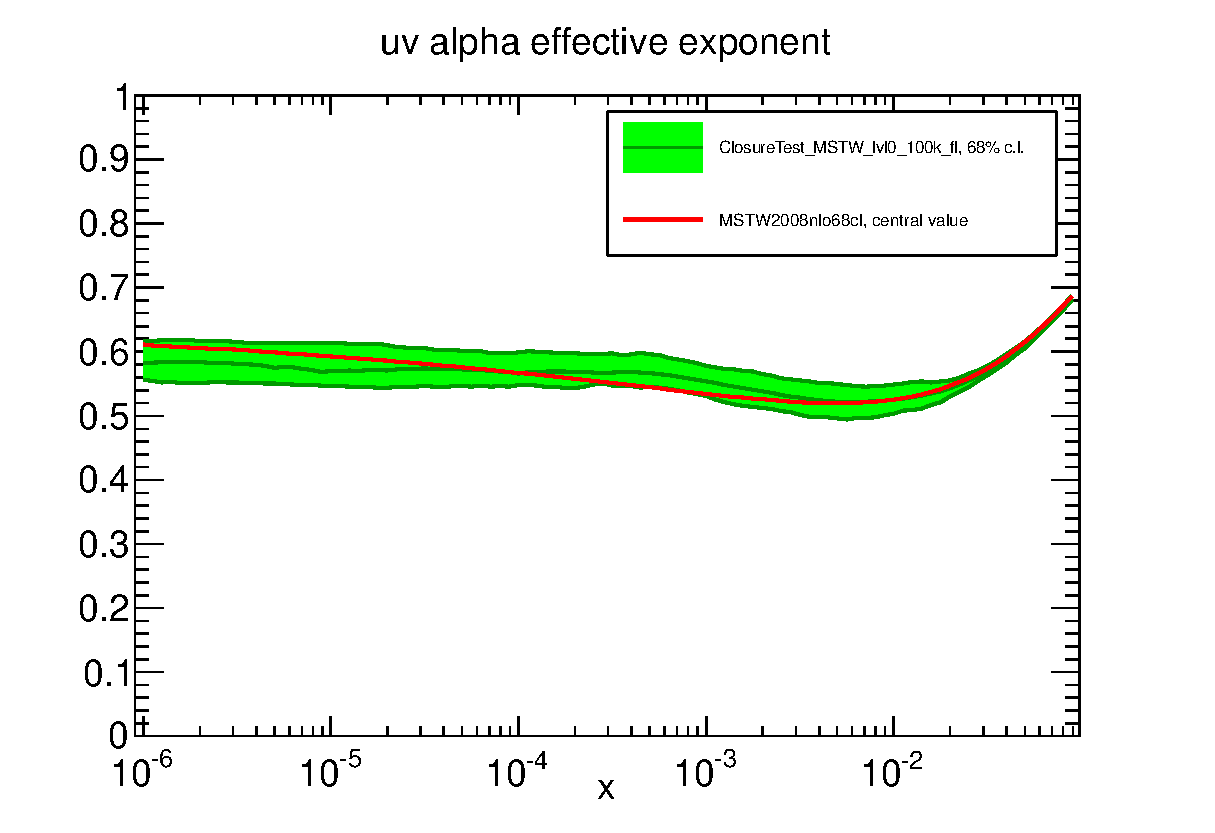
\includegraphics[width=0.5\textwidth]{figures/uv_preproc_CT_vs_MSTW_alpha.eps}
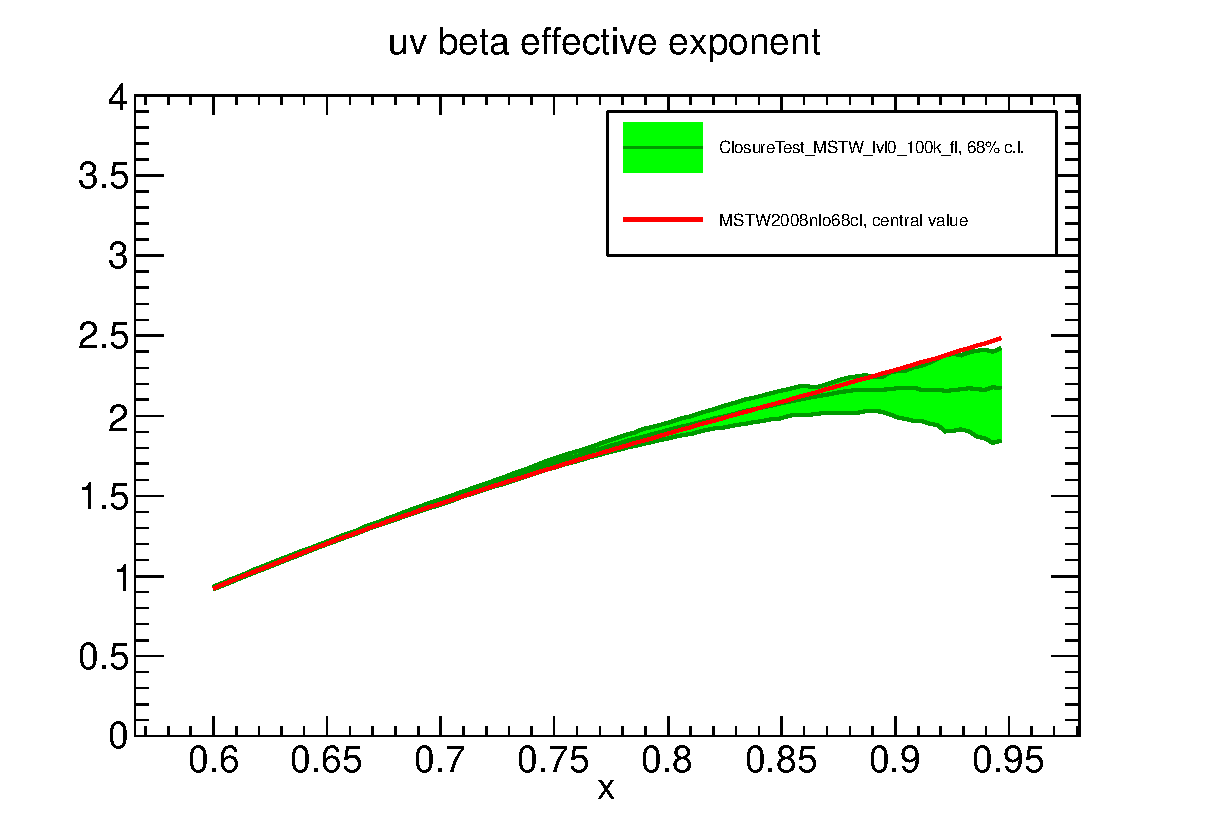
\includegraphics[width=0.5\textwidth]{figures/uv_preproc_CT_vs_MSTW_beta.eps}

\end{center}

\end{frame}


%%%%%%%%%%%%%%%%%%%%%%%%%%%%%%%%%%%%%%%%%%%%%%%%%%%%%%%%%
\begin{frame}
\frametitle{Level two closure tests}
\begin{itemize}
\item Ideal pseudodata $\to$ simulate noise $\to$ generate artificial data.
\end{itemize}
\includegraphics[width=0.5\textwidth]{figures/gluon.pdf}
\includegraphics[width=0.5\textwidth]{figures/singlet.pdf}

\underline{Important test}\\
Are the stated uncertainties reliable? $\to$ Examine the fraction $\xi$ of fits where the input PDF set falls into the 1-$\sigma$/ 2-$\sigma$ band.\\
\vskip 10pt
\textbf{Level one} CT:  $\xi_{1\sigma} = 0.512, \quad \xi_{2\sigma} = 0.836$. \\
\textbf{Level two} CT:   $\xi_{1\sigma} = 0.699, \quad \xi_{2\sigma} = 0.948$. \\
\textbf{Gaussian} Ideal: $\xi_{1\sigma} = 0.68, \quad \xi_{2\sigma} = 0.95$.
\end{frame}



%%%%%%%%%%%%%%%%%%%%%%%%%%%%%%%%%%%%%%%%%%%%%%%%%%%%%%%%%
\begin{frame}
\frametitle{Level two closure tests - $\chi^2$ reproduction}
\underline{How do we do when it comes to the \textbf{data description?} }\\

\begin{itemize}
\item Compare the $\chi^2$ of CT fit to the $\chi^2$ of the underlying PDF.
\end{itemize}

\begin{center}
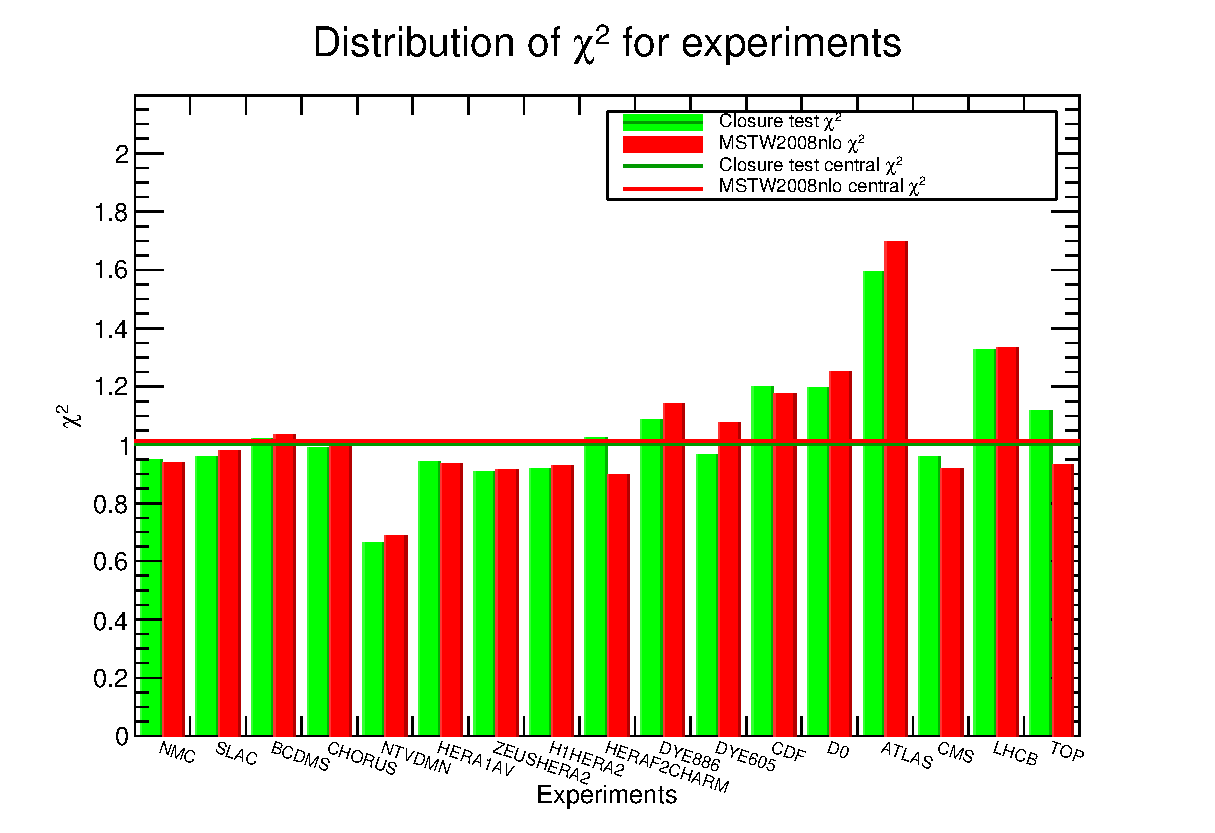
\includegraphics[width=0.8\textwidth]{figures/Chi2Histo_CT_vs_MSTW.eps}
\end{center}

\end{frame}

%%%%%%%%%%%%%%%%%%%%%%%%%%%%%%%%%%%%%%%%%%%%%%%%%%%%%%%%%
\begin{frame}
\frametitle{Breakdown of uncertainties}
\begin{center}
\underline{Closure tests can provide information on the breakdown of uncertainties}
\end{center}
\begin{itemize}
\item Level zero - inter/extrapolation uncertainties
\item Level one - functional uncertainties
\item Level two - experimental data uncertainties
\end{itemize}

\begin{center}
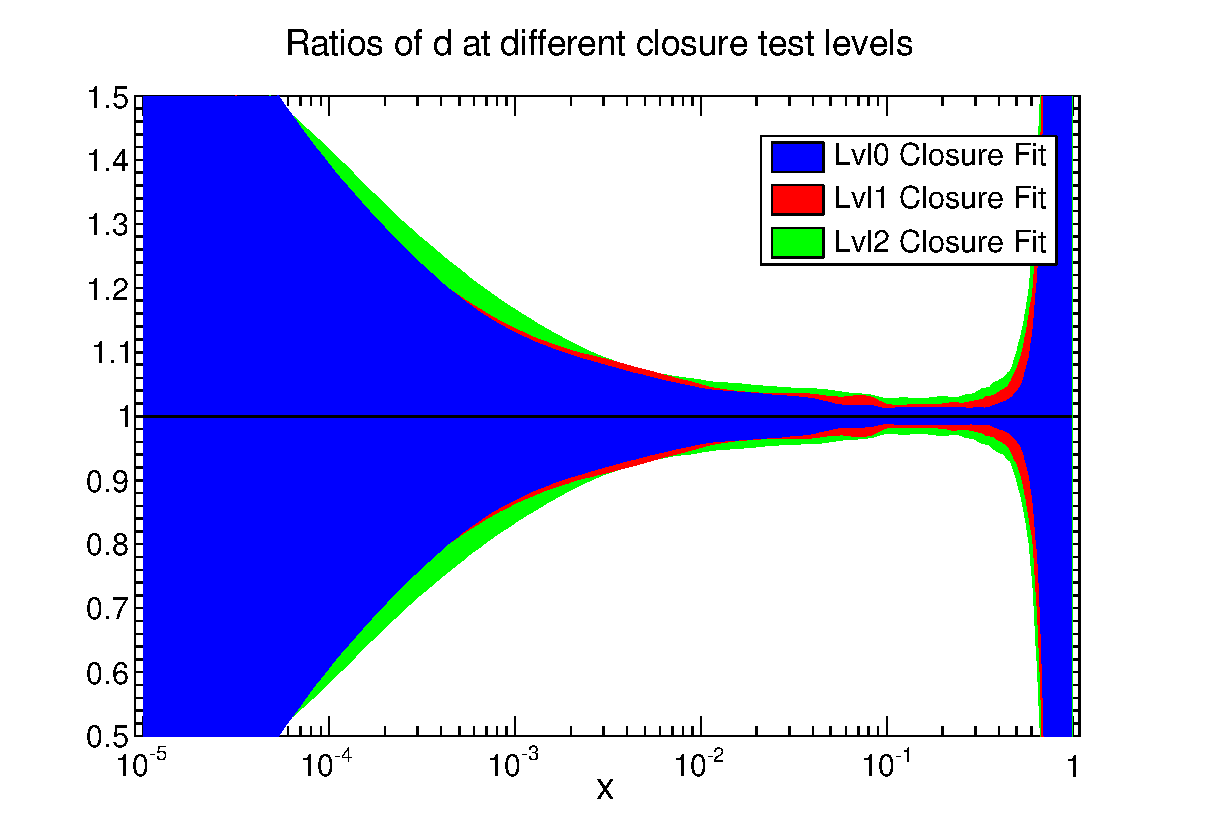
\includegraphics[width=0.5\textwidth]{figures/CT123ratios_d.eps}
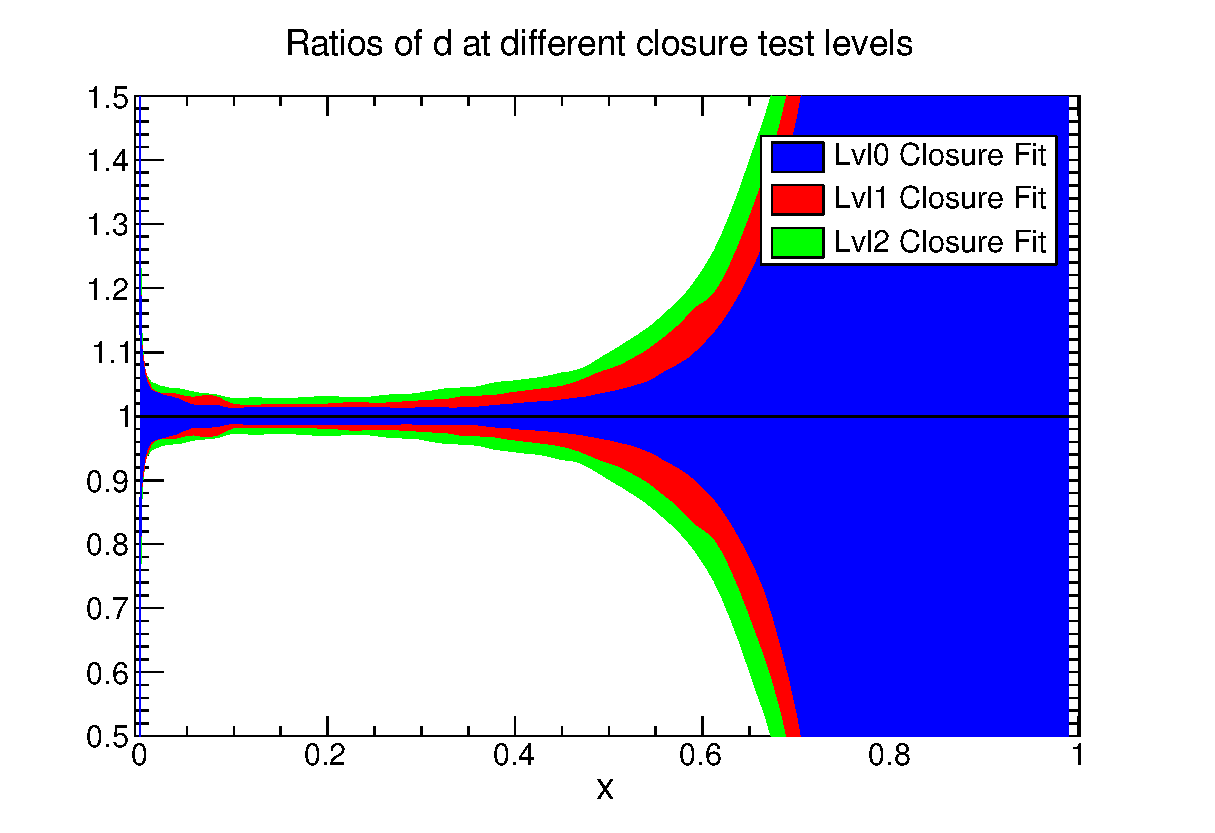
\includegraphics[width=0.5\textwidth]{figures/CT123ratios_d_lin.eps}

\textbf{Pseudodata fits could provide information on optimal data binning?}
\end{center}

\end{frame}

%%%%%%%%%%%%%%%%%%%%%%%%%%%%%%%%%%%%%%%%%%%%%%%%%%%%%%%%%
\begin{frame}
\frametitle{PDFs for the second run of the LHC}
\textbf{Improvements for NNPDF3.0}
\vskip10pt
\underline{Closure tests provided us with plenty to learn from}
\begin{itemize}
\item Newer genetic algorithm - \emph{Faster and more effective fits}.
\item Improved preprocessing - \emph{Iterative method minimises bias}
\item Simpler fitting procedure  
\end{itemize}
\vskip15pt
\textbf{Provided a detailed validation of fitting efficiency, and PDF uncertainties.}
\vskip15pt
\underline{Other improvements}
\begin{itemize}
\item Expanded set of positivity observables.
\item EW corrections to LHC DY
\item Improved understanding of Jet data at NNLO
\end{itemize}

\end{frame}

%%%%%%%%%%%%%%%%%%%%%%%%%%%%%%%%%%%%%%%%%%%%%%%%%%%%%%%%%
\begin{frame}
\frametitle{The NNPDF3.0 PDF set}

\includegraphics[width=0.50\textwidth]{figures/xg-abs-30_vs_23_lowscale.eps}
\includegraphics[width=0.50\textwidth]{figures/xsinglet-abs-30_vs_23_lowscale.eps}\\
\includegraphics[width=0.50\textwidth]{figures/xtriplet-abs-30_vs_23_lowscale.eps}
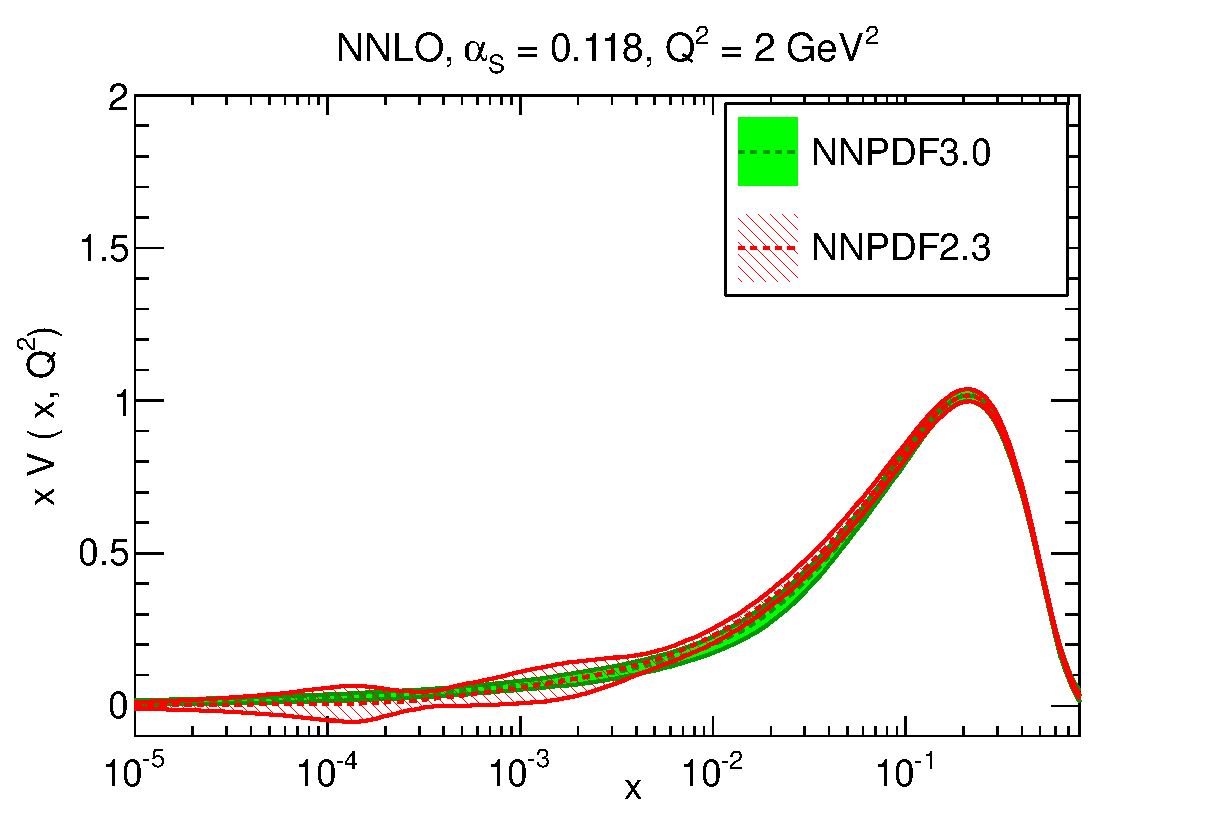
\includegraphics[width=0.50\textwidth]{figures/xvalence-abs-30_vs_23_lowscale.eps}


\end{frame}

%%%%%%%%%%%%%%%%%%%%%%%%%%%%%%%%%%%%%%%%%%%%%%%%%%%%%%%%%
\begin{frame}
\frametitle{Impact of LHC data}

\includegraphics[width=0.50\textwidth]{figures/xu-30_vs_noLHC_highscale.eps}
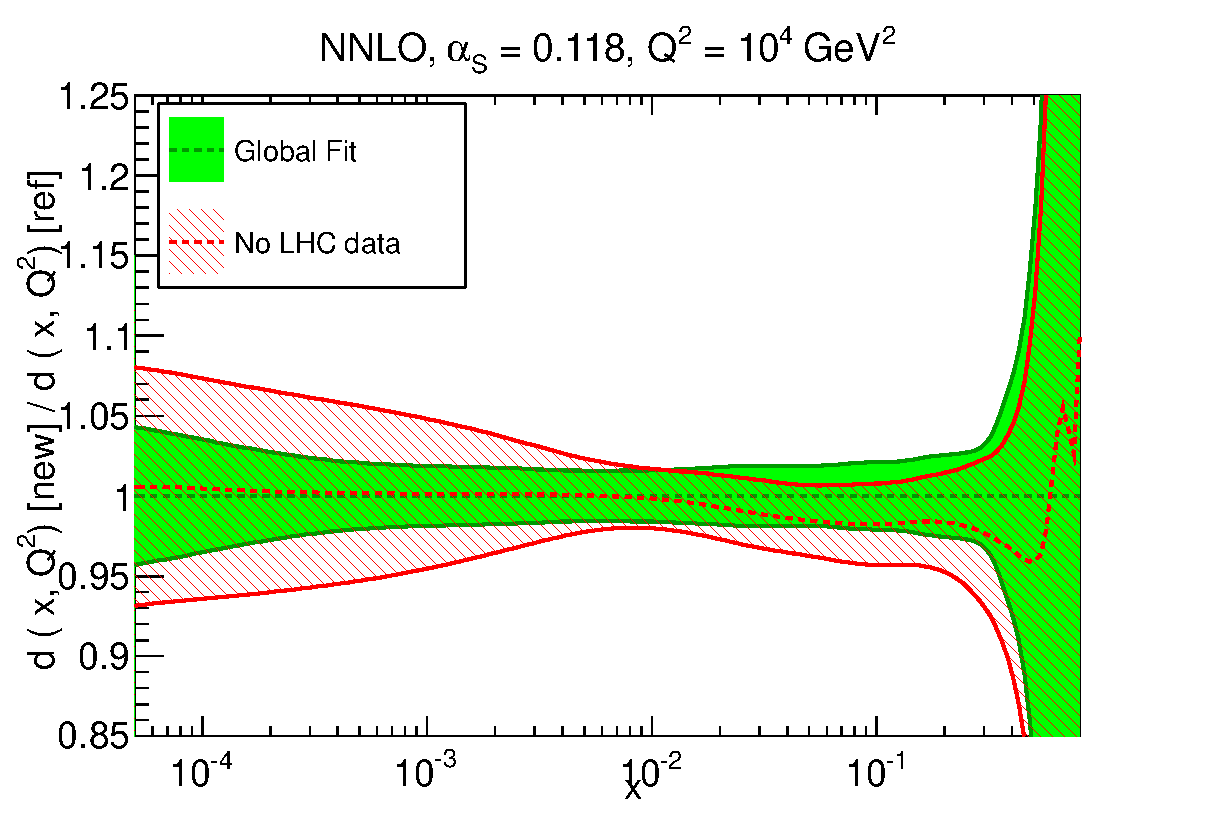
\includegraphics[width=0.50\textwidth]{figures/xd-30_vs_noLHC_highscale.eps}\\
\includegraphics[width=0.50\textwidth]{figures/xg-30_vs_noLHC_highscale.eps}
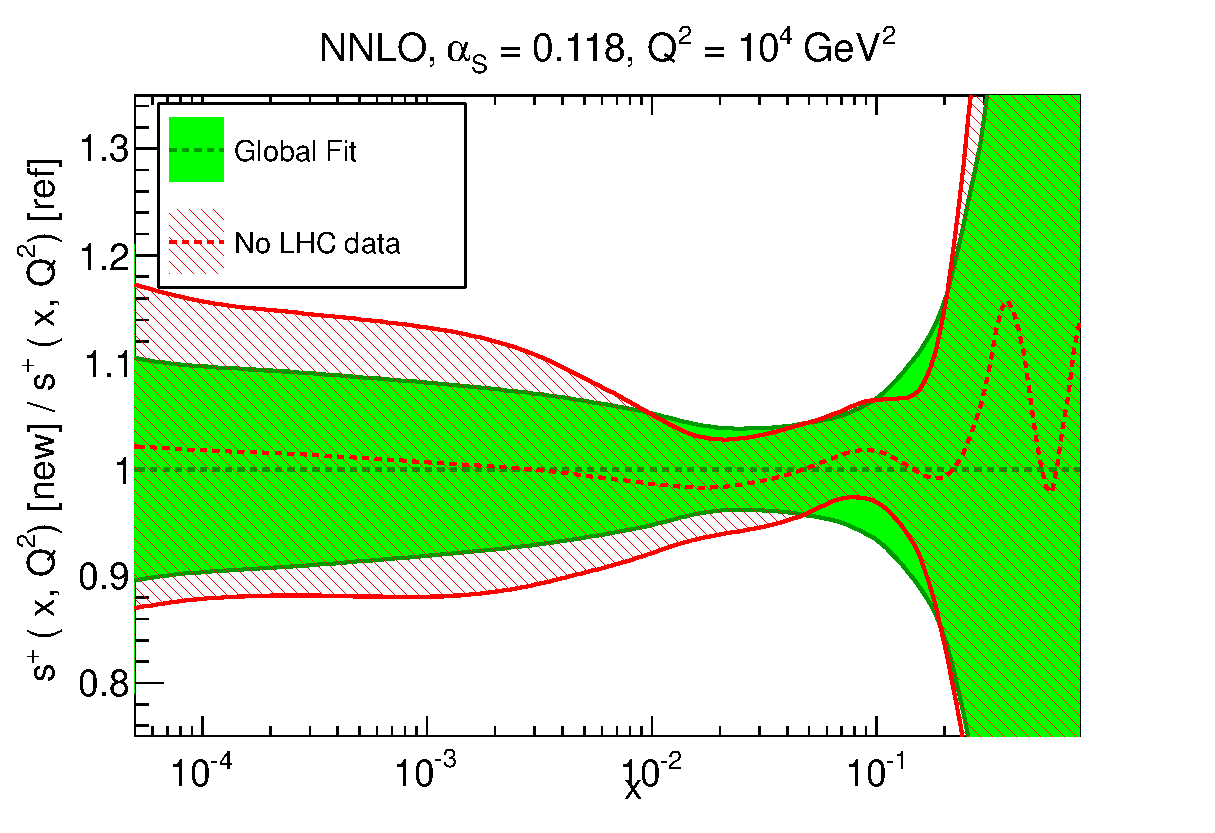
\includegraphics[width=0.50\textwidth]{figures/xsp-30_vs_noLHC_highscale.eps}

\end{frame}

%%%%%%%%%%%%%%%%%%%%%%%%%%%%%%%%%%%%%%%%%%%%%%%%%%%%%%%%%


\begin{frame}
\frametitle{NNPDF3.0 data description}

\begin{center}
\begin{tabular}{c||ccc|ccc}
\hline
 & \multicolumn{3}{c}{NLO} & \multicolumn{3}{c}{NNLO} \\
\hline
 &  $N_{\rm dat}$  & $\chi^{2}_{\rm exp}$ & $\chi^{2}_{\rm t_0}$ & $N_{\rm dat}$  & $\chi^{2}_{\rm exp}$ & $\chi^{2}_{\rm t_0}$ \\
\hline
\hline
Total   & 4276 	& 1.23  & 1.25 & 4078 	& 1.29 & 1.27 \\
\hline
\hline
ATLAS $W,Z$ 2010   & 30 & 1.19 & 1.25 & 30 & 1.23 & 1.18\\
ATLAS 7 TeV jets 2010    & 90 & 1.07 & 0.52 & 9 & 1.36 & 0.85\\
ATLAS 2.76 TeV jets  & 59 & 1.29 & 0.65 & 3 & 0.33 & 0.33\\
ATLAS high-mass DY  & 5 & 2.06 & 2.84 & 5 & 1.45 & 1.81\\
ATLAS $W$ $p_T$  &   9 & 1.13 & 1.28 & - & - & - \\
CMS $W$ electron asy   & 11 & 0.87 & 0.79 & 11 & 0.73 & 0.70\\
CMS $W$ muon asy   & 11 & 1.81 & 1.80 & 11 & 1.72 & 1.72\\
CMS jets 2011   & 133 & 0.96 & 0.91 & 83 & 1.9 & 1.07\\
CMS $W+c$ total   & 5 & 0.96 & 1.30 & 5 & 0.84 & 1.11\\
CMS $W+c$ ratio   & 5 & 2.02 & 2.02 & 5 & 1.77 & 1.77\\
CMS 2D DY 2011   & 88 & 1.23 & 1.56 & 110 & 1.36 & 1.59\\
LHCb $W$ rapidity   & 10 & 0.71 & 0.69 & 10 & 0.72 & 0.63\\
LHCb $Z$ rapidity   & 9 & 1.10 & 1.34 & 9 & 1.59 & 1.80\\
$\sigma(t\bar{t})$  & 6 & 1.43 & 1.68 & 6 & 0.66 & 0.61\\
\hline
\hline
\end{tabular}
\end{center}



 \end{frame} 



%%%%%%%%%%%%%%%%%%%%%%%%%%%%%%%%%%%%%%%%%%%%%%%%%%%%%%%%%
\begin{frame}
\frametitle{ NNPDF HERA only fits }

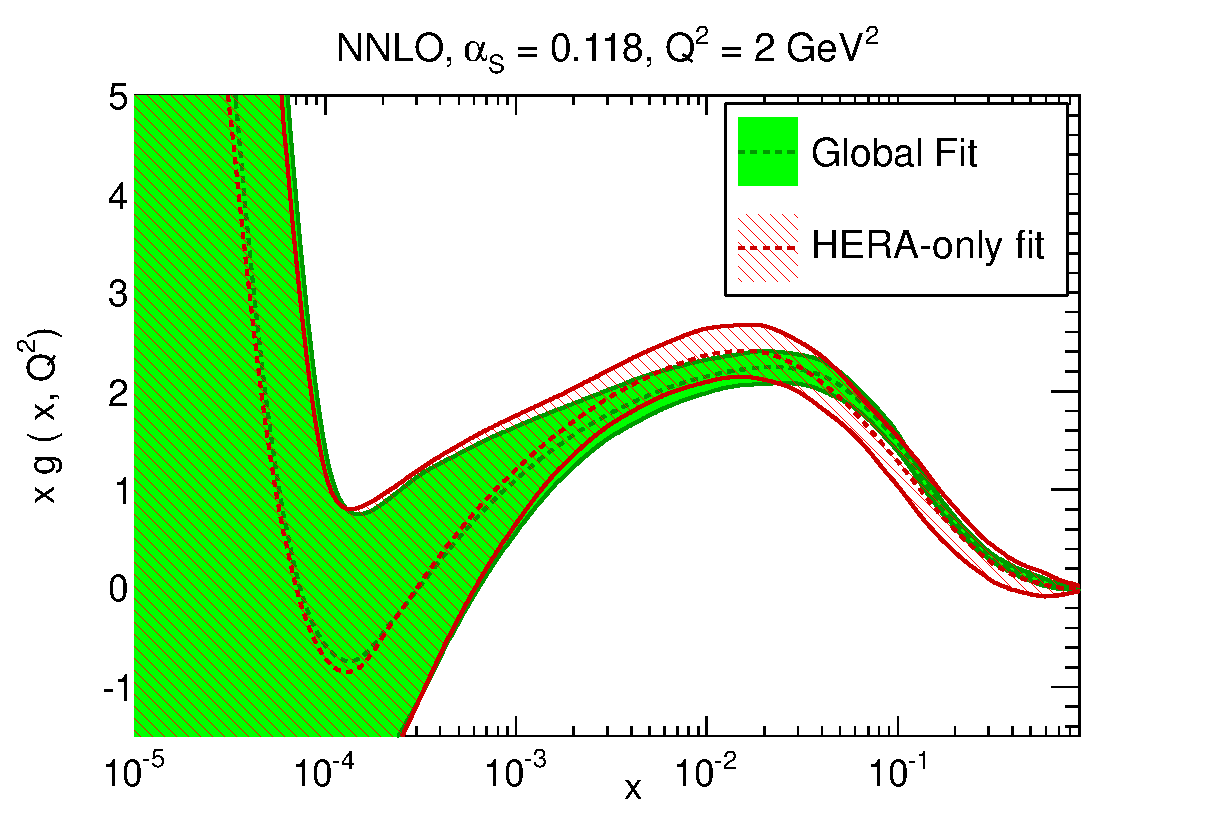
\includegraphics[width=0.50\textwidth]{figures/xg-abs-30_vs_heraonly.eps}
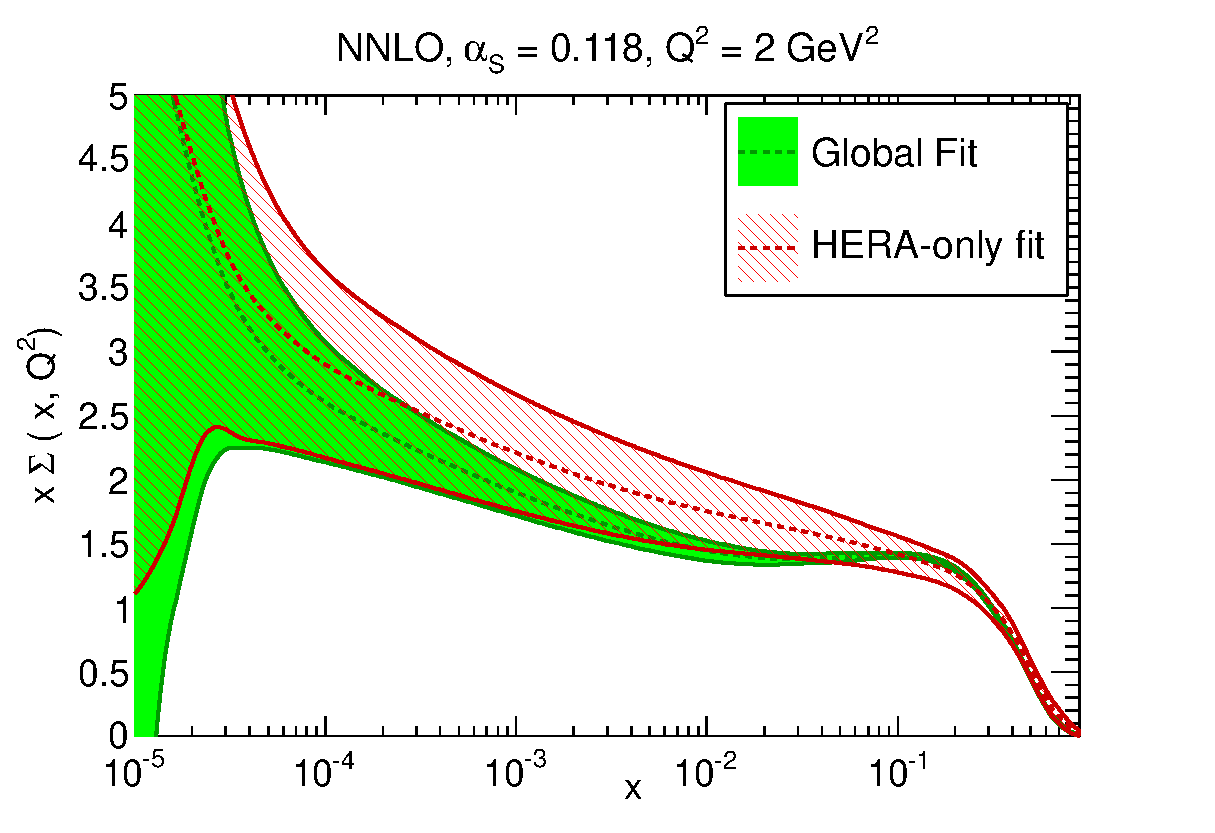
\includegraphics[width=0.50\textwidth]{figures/xsinglet-abs-30_vs_heraonly.eps}\\
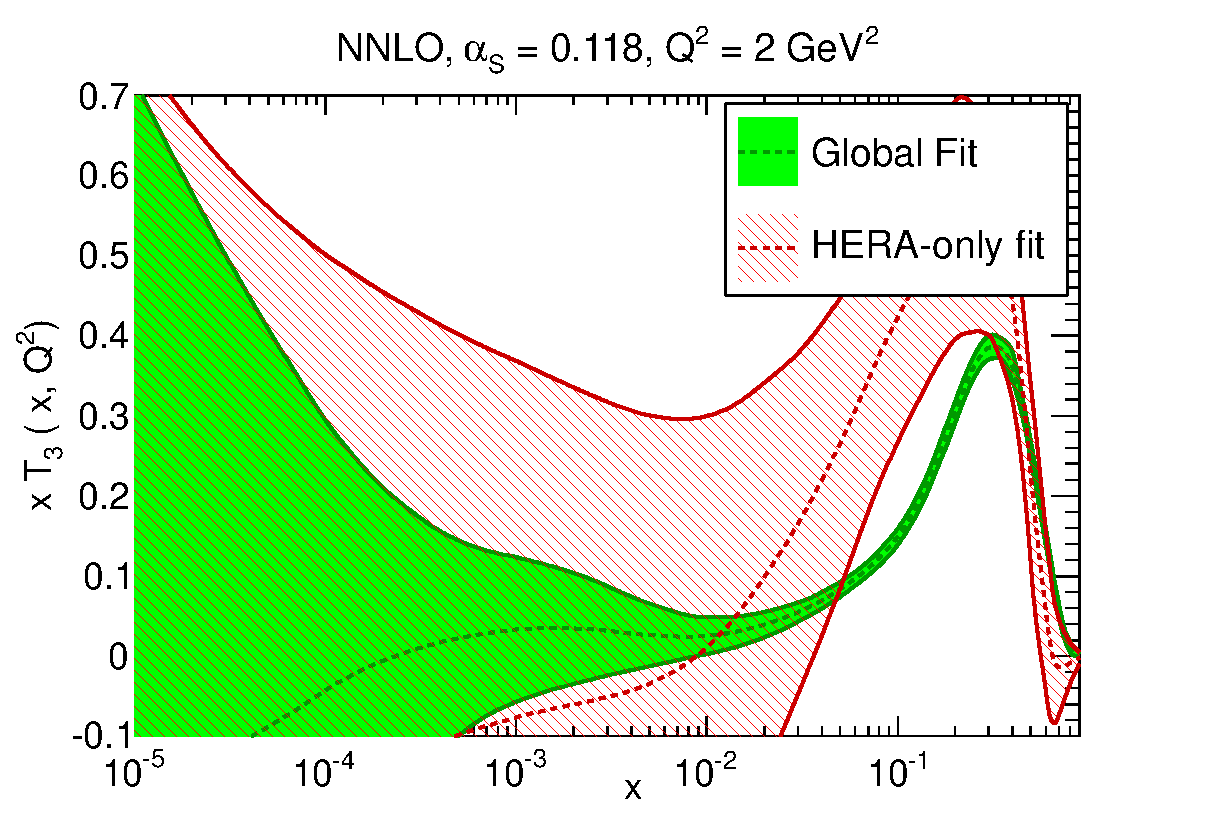
\includegraphics[width=0.50\textwidth]{figures/xtriplet-abs-30_vs_heraonly.eps}
\includegraphics[width=0.50\textwidth]{figures/xvalence-abs-30_vs_heraonly.eps}
\end{frame}


%%%%%%%%%%%%%%%%%%%%%%%%%%%%%%%%%%%%%%%%%%%%%%%%%%%%%%%%%
\begin{frame}
\frametitle{ Conclusion }
\underline{Precise and reliable PDFs are vital for physics at the LHC}

\begin{itemize}
\item Robust fitting methodology is essential.
\item An understanding of the basis of PDF uncertainties is important.
\item Fits to a large, global dataset (including LHC data) remain crucial.
\end{itemize}
\vskip15pt

\begin{center}
\textbf{Closure tests enabled detailed validation of methodology in NNPDF3.0.}
\textbf{Fast interfaces, and the FK method allow an enlarged dataset.}
\end{center}

\vskip15pt
\underline{LHC data has the potential to answer a lot of open questions in proton structure}
\begin{itemize}
\item How important are strange quark distributions?
\item Are low-energy, fixed target datasets consistent?
\item How reliable are deuteron/nuclear corrections?
\end{itemize}

\end{frame}


%%%%%%%%%%%%%%%%%%%%%%%%%%%%%%%%%%%%%%%%%%%%%%%%%%%%%%%%%%%%%
%%%%%%%%%%%%%%%%%%%%%%%%%%%%%%%%%%%%%%%%%%%%%%%%%%%%%%%%%%%%%


\begin{frame}
    \begin{center}
      BACKUPS
    \end{center}
\end{frame}

%%%%%%%%%%%%%%%%%%%%%%%%%%%%%%%%%%%%%%%%%%%%%%%%%%%%%%%%%%%%%
\begin{frame}
    \begin{center}
\frametitle{Electroweak corrections in NNPDF3.0}
      \includegraphics[width=0.4\textwidth]{figures/atlasHM.eps}
      \includegraphics[width=0.4\textwidth]{figures/bin1cms.eps}
    \end{center}
\end{frame}


%%%%%%%%%%%%%%%%%%%%%%%%%%%%%%%%%%%%%%%%%%%%%%%%%%%%%%%%%


\begin{frame}
\frametitle{The strange content of the proton.}

    \begin{columns}
  \begin{column}{0.5\textwidth}
  \begin{center} 
     \includegraphics[width=0.8\textwidth]{figures/fig2.pdf}\\
       \includegraphics[width=0.8\textwidth]{figures/rs-2.eps}
       \end{center}
               \end{column}
  \begin{column}{0.5\textwidth}
  
    \begin{center} 

   \includegraphics[width=0.9\textwidth]{figures/CMSWc.png}
       \end{center}

   \end{column}
  \end{columns}
            \vskip10pt
  {\small
  \begin{itemize}
\item<1->NNPDF fit to HERA and ATLAS-WZ data finds central
value consistent with ATLAS\footnote{arXiv:1203.4051} determination of $r_s(x) = (s(x) + \bar{s}(x)) / 2d(x)$ within a large uncertainty.
\item<1->Recent CMS\footnote{CMS-SMP-12-002} measurement of $W+c$ consistent with strangeness in global fits.
Slightly disfavours the larger strange sea in NNPDF2.3 Collider only, but consistent within uncertainties.
\end{itemize}

}

\end{frame}


%%%%%%%%%%%%%%%%%%%%%%%%%%%%%%%%%%%%%%%%%%%%%%%%%%%%%%%%%


\begin{frame}
\frametitle{NNPDF2.3 Collider only vs NNPDF2.3}
   \includegraphics[width=0.5\textwidth]{figures/xg_Q_2_log-23-vs-23coll-nnlo.eps}
 \includegraphics[width=0.5\textwidth]{figures/xSinglet_Q_2_log-23-vs-23coll-nnlo.eps}\\
    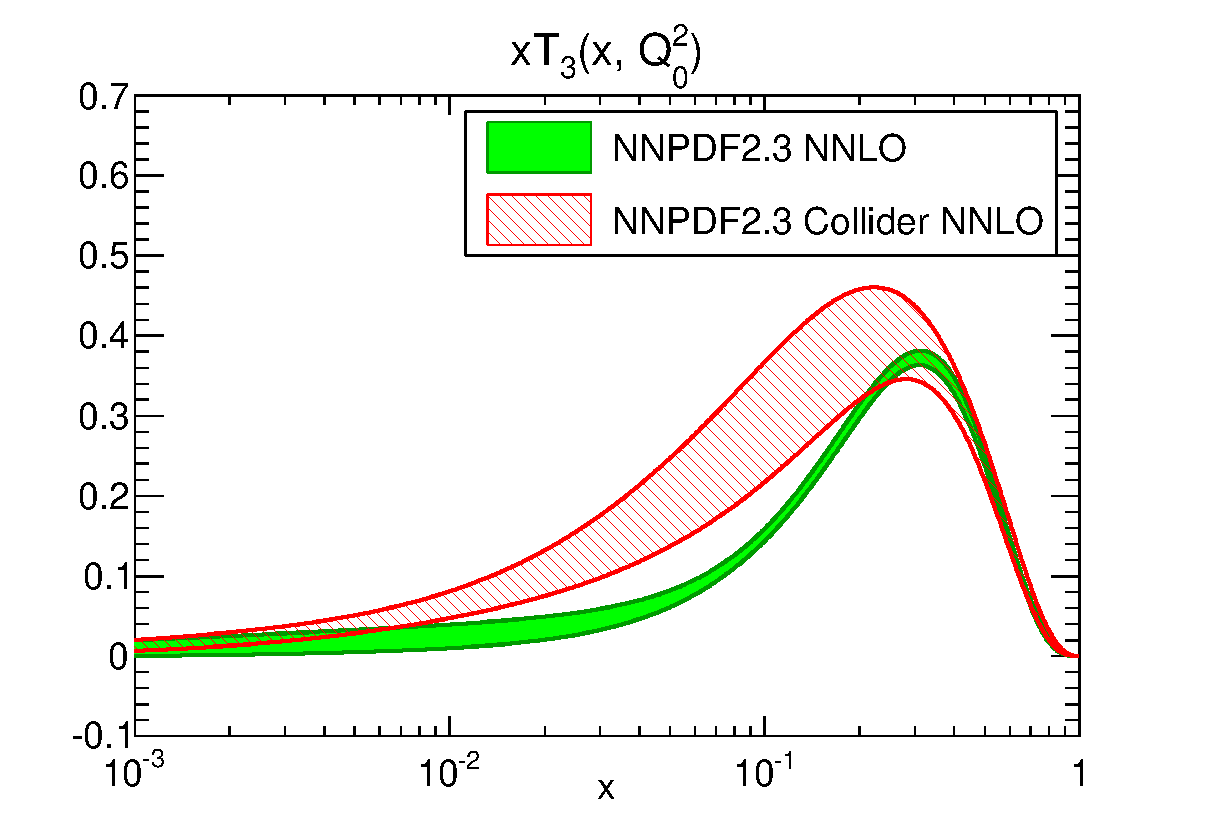
\includegraphics[width=0.5\textwidth]{figures/xT3_Q_2_log-23-vs-23coll-nnlo.eps}
 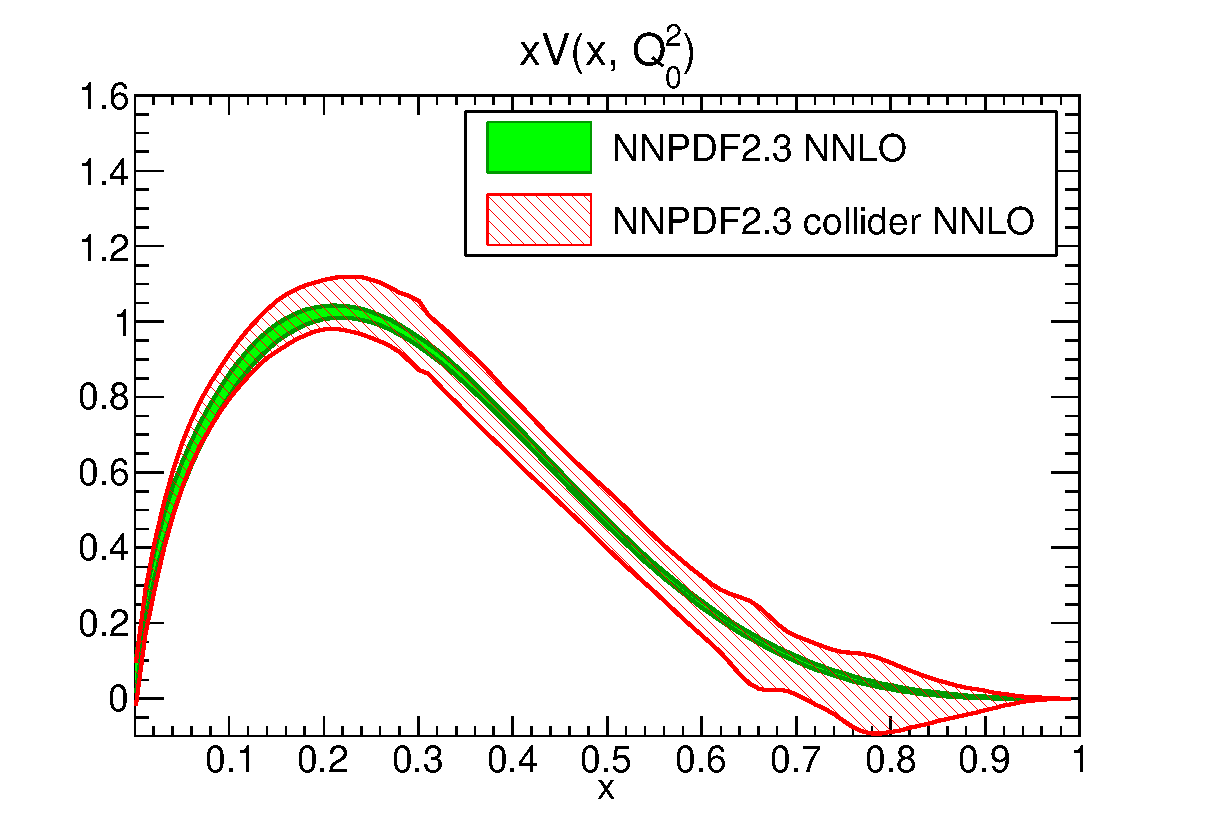
\includegraphics[width=0.5\textwidth]{figures/xV_Q_2_lin-23-vs-23coll-nnlo.eps}
 \end{frame} 

%%%%%%%%%%%%%%%%%%%%%%%%%%%%%%%%%%%%%%%%%%%%%%%%%%%%%%%%%

\begin{frame}
\frametitle{t0 method - closure tests}
   \includegraphics[width=0.9\textwidth]{figures/t0plot.pdf}
 \end{frame} 

%%%%%%%%%%%%%%%%%%%%%%%%%%%%%%%%%%%%%%%%%%%%%%%%%%%%%%%%%
\begin{frame}
\frametitle{Including new experimental data}
How can we add new data to an existing parton set?

\begin{itemize}
		\item<1-> Perform a new fit.\\
		{\small (Difficult if a fast implementation of the theoretical prediction is not available).}
		\item<1-> Reweight existing Monte Carlo parton set. {\small \color{blue} Giele, Keller [hep-ph/9803393] }\\
\end{itemize}
If the new data is statistically independent of the data in the prior set:
\be
\mathcal{P}_{\rm new}(f)
= \mathcal{N}_{\chi}\mathcal{P}(\chi^2|f)\;\mathcal{P}_{\rm old}(f),
\ee
		\be \langle\mathcal{O}\rangle_{\mathrm {new}}=\int \mathcal{O}[f] \, \mathcal{P}_{ \mathrm {new}}(f)\,Df=\smallfrac{1}{N}\,\sum_{k=1}^{N}w_k\mathcal{O}[f_k].\,  \ee
Weights determined by statistical inference
\be w_k =\mathcal{N}_\chi\mathcal{P}(\chi^2|f_k) = 
\frac{(\chi^{2}_k)^{(n-1)/2} 
e^{-\frac{1}{2}\chi^{2}_k}}
{\smallfrac{1}{N}\sum_{k=1}^{N}(\chi^{2}_k)^{(n-1)/2}
e^{-\frac{1}{2}\chi^{2}_k}}\, .\ee
\center{ \small  R.~D.~Ball {\it et al.} Nucl.\ Phys.\ B {\bf 849} 112  [arXiv:1012.0836]. }

\end{frame}

%%%%%%%%%%%%%%%%%%%%%%%%%%%%%%%%%%%%%%%%%%%%%%%%%%%%%%%%%
\begin{frame}
\frametitle{Error rescaling parameter}
Useful tool for analysing experimental uncertainties. 
Differentiates between inconsistent and constraining data when $N_{\mathrm{eff}}$ is small.
\begin{itemize}
		\item<1-> Rescale uncertainties by a factor $\alpha$.
		\item<1-> Compute a new weight $w_k(\alpha)$ with these uncertainties.
		\item<1-> Average over all replicas $\to$ probability of rescaling uncertainties by $\alpha$.
\end{itemize}


\begin{columns}
  \begin{column}{0.5\textwidth}
  \begin{block}{}
\be \chi^2_{k,\alpha} = \chi^2_k/\alpha^2, \ee
\be w_k(\alpha) = (\chi^2_{k,\alpha})^{(n-1)/2}\mathrm{e}^{-\chi^2_{k,\alpha}/2,}\ee
\be \mathcal{P}(\alpha | \chi^2)\propto \smallfrac{1}{\alpha}\sum_{k=1}^N w_k(\alpha).\ee
\end{block}
  \end{column}
  
    \begin{column}{0.5\textwidth}
 \begin{figure}[b!]
    \begin{center}
      \includegraphics[width=1\textwidth]{figures/palpha-jets-t0.eps}
    \end{center}
\end{figure}

  \end{column}  
  \end{columns}

\begin{figure}[b!]
    \begin{center}
    \end{center}
    \vskip-0.5cm

\end{figure}

\end{frame}



% End of slides
\end{document} 